\documentclass[12pt, openany]{book}

% !TEX root=../../mt-motion-analysis.tex
\usepackage[citestyle=ieee, bibstyle=ieee, style=numeric-comp, sorting=nty, maxbibnames=99]{biblatex}

\usepackage[utf8]{inputenc}

% Makes the last name first in the bibliography.
% \DeclareNameAlias{author}{last-first}
% \DeclareNameAlias{author}{family-given}

% Specify the margins. This is 6.25inches in text with which
% can be used to size figures to the correct size.
\usepackage[a4paper, margin=2.5625cm]{geometry}


\usepackage{eso-pic}					% Packages for layout and graphics
\usepackage{graphicx}
\usepackage{tikz}
\usetikzlibrary{fadings}
\usepackage{setspace}
% \usepackage{tocloft}		 			% Fixing a bug with page style changes for toc
% \tocloftpagestyle{plain}
\usepackage{etoc} 						% Separate tocs for appendix and the rest
\usepackage{chngcntr}					% Count figures within chapters
\usepackage{booktabs}					% Table formatting
\usepackage{fancyhdr}					% Setting the style for header and footer.
\usepackage{tabularx}
\usepackage{multirow}                   % For better tables
\usepackage[hidelinks]{hyperref}		% Clickable links
\usepackage{nameref}					% References with names
\usepackage[parfill]{parskip}			% New line instead of indent for sections
\usepackage{tcolorbox}					% Create boxes around content
\tcbset{colback=white,arc=0mm}

\usepackage{amsmath}
\usepackage{mathdots}
\usepackage{yhmath}
\usepackage{siunitx}
\usepackage{array}
\usepackage{gensymb}
\usepackage{amssymb}
\usepackage{mathtools}              % Add text to math arrows.

\usepackage{cancel}
\usepackage{color}
\usepackage{multirow}
\usepackage{textcomp}               % Fixing warning for gensyb \perthousand
\usepackage{svg}                    % including svg files
\usepackage{caption}                % For subfigures
\usepackage{subcaption}
\usepackage{fontspec}
\usepackage{sectsty}
\usepackage{tocloft}

\usepackage[printonlyused]{acronym}

\usepackage{slashbox}
\usepackage{arydshln}

\usepackage{cleveref}

\usepackage{unicode-math}

% \usepackage{bm}

\usepackage[acronym, nonumberlist, nopostdot, xindy, nomain, nogroupskip]{glossaries}





\counterwithin{figure}{section}
\counterwithin{table}{section}

% Specifying fonts
% \setmainfont{Georgia}
% \setsansfont{Arial}
% \newfontfamily\footerfont{Georgia}

\chapterfont{\sffamily\fontsize{17}{17}}
\sectionfont{\sffamily\fontsize{14}{15}}
\subsectionfont{\sffamily\fontsize{13}{15}}
\subsubsectionfont{\sffamily\fontsize{12}{15}}

% Remove the title and make sure that the text is adjusted
% \usepackage{abstract}
% \setlength{\absleftindent}{0mm}
% \renewcommand{\abstractname}{\vspace{-\baselineskip}}
% \renewcommand{\abstractnamefont}{\sffamily\fontsize{14}{15}}
% \renewcommand{\abstracttextfont}{\normalfont\fontsize{12}{13}}

% Renaming and setting style of table of contents
\renewcommand*\contentsname{Contents}
\renewcommand*\cfttoctitlefont{\fontsize{16}{0}\bf\sffamily}
\renewcommand\cftchapfont{\fontsize{14}{0}\bf\sffamily}
\renewcommand\cftchappagefont{\fontsize{13}{0}\bf\sffamily}
\renewcommand\cftsecfont{\fontsize{12}{0}\sffamily}
\renewcommand\cftsecpagefont{\fontsize{12}{0}\sffamily}
\renewcommand\cftsubsecfont{\fontsize{12}{0}\sffamily}
\renewcommand\cftsubsecpagefont{\fontsize{12}{0}\sffamily}

% Styling the header and footer
\fancyhf{}
\fancyhead{}
\fancyfoot{}
\fancyhead[L]{\fontsize{11}{10}\selectfont\leftmark}
\fancyfoot[R]{\footerfont\thepage}
\setlength{\headheight}{15.5pt}




\fancypagestyle{plain}{
 \fancyhf{}
 \fancyhead{}
 \fancyfoot{}
 \renewcommand{\headrulewidth}{0pt}
 \fancyfoot[R]{\footerfont\thepage}
}

\pagestyle{fancy}

% Making the command for placing text in random locations
\newcommand\PlaceText[3]{%
 \begin{tikzpicture}[remember picture,overlay]
  \node[outer sep=0pt,inner sep=0pt,anchor=south west]
  at ([xshift=#1,yshift=-#2]current page.north west) {#3};
 \end{tikzpicture}%
}

% Disable hyphenation
\pretolerance=10000
\tolerance=2000
\emergencystretch=50pt

% !TEX root=../mt-motion-analysis.tex
\newtheorem{definition}{Definition}

\newsavebox{\mybox}

\xdef\myspbetween{0.25cm}

% \newenvironment{definition}[1][]
% {\savebox\mybox{\hbox{Definition \thetheorem}}%
% \xdef\mdim{\the\dimexpr\wd\mybox+10pt}%
% \xdef\mybdim{\the\dimexpr\textwidth-\mdim-\myspbetween}%
% \noindent\begin{minipage}[t]{\mdim}%
% \begin{olddefinition}[#1]\end{olddefinition}\end{minipage}\hspace{\fill}\begin{minipage}[t]{\mybdim}}
% {\end{minipage}\medskip}


\newtheorem{theorem}{Theorem}
\newenvironment{myTheorem}[1][]
{\savebox\mybox{\hbox{Theorem \thetheorem}}%
\xdef\mdim{\the\dimexpr\wd\mybox+10pt}%
\xdef\mybdim{\the\dimexpr\textwidth-\mdim-\myspbetween}%
\noindent\begin{minipage}[t]{\mdim}%
\begin{theorem}[#1]\end{theorem}\end{minipage}\hspace{\fill}\begin{minipage}[t]{\mybdim}}
{\end{minipage}\medskip}

\newenvironment{conditions}[1][where:]
  {#1 \begin{tabular}[t]{>{$}l<{$} @{} >{${}}c<{{}$} @{} l}}
  {\end{tabular}\\[\belowdisplayskip]}

% !TEX root=../mt-motion-analysis.tex

\newcommand*\mean[1]{\mathop{\overline{#1}}}

\makeglossaries
\setacronymstyle{long-short}
\newacronym{mpii}{MPII}{Max Planck Institute for Informatics dataset}
\newacronym{coco}{COCO}{Microsoft Common Objects in Context dataset}
\newacronym{aic-hkd}{AIK-HKD}{AI Challenger Human
Keypoint Detection dataset}
\newacronym{coco-whole}{COCO-wholebody}{Microsoft Common Objects in Context wholebody dataset}
\newacronym{hpe}{HPE}{Human Pose Estimation}
\newacronym{cnn}{CNN}{Convolutional Neural Network}
\newacronym{sota}{SOTA}{State of the Art}
\newacronym{dnn}{DNN}{Deep Neural Network}
\newacronym{hrnet}{HRNet}{High-Resolution Net}
\newacronym{dark}{DARK}{Distribution-Aware coordinate Representation of Key-point}
\newacronym{tsc}{TSC}{Time Series Classification}
\newacronym{cote}{COTE}{Collective Of Transformation-based Ensembles}
\newacronym{hive-cote}{HIVE-COTE}{Hierarchical Vote Collective of Transformation-based Ensembles }
\newacronym{ucr}{UCR}{University of California, Riverside}
\newacronym{gap}{GAP}{Global Average Pooling}
\newacronym{grad-cam}{Grad-CAM}{Gradient-weighted Class Activation Mapping}
\newacronym{coral}{CORAL}{COnsistent RAnk Logits}
\newacronym{gpu}{GPU}{Graphics Processing Unit}
\newacronym{relu}{ReLU}{Rectified Linear Unit}
\newacronym{poe}{POE}{Postural Orientation Error}
\newacronym{sls}{SLS}{Single Leg Squat}
\newacronym{xcm}{XCM}{Explainable Convolutional Neural Network for Multivariate
Time Series Classification}
\newacronym{acl}{ACL}{Anterior Cruciate Ligament}
\newacronym{ai}{AI}{Artificial Intelligence}


% \bibliography{files/bibtex/bib}
% \bibliography{files/bib}
\addbibresource{files/bibtex/bib.bib}

% \title{POE assessments of movements using deep learning}
\title{Assessments of Posterior Orientation Errors after Anterior Cruciate Ligament injuries using deep learning based methods}
% \title{Assessment of rehabilitation after Anterior Cruciate Ligament injuries using deep learning based methods}
\author{Filip Kronström}
\date{\today}


% \includeonly{files/text/0-pre-content, files/text/3-related-work-tsc}
\begin{document}
\setstretch{0.9}
\maketitle
\pagenumbering{roman}
% !TEX root=../../mt-motion-analysis.tex
% \newpage
% Anterior Cruciate Ligament (ACL)
\tableofcontents
\chapter*{Abstract}
\addcontentsline{toc}{chapter}{Abstract}
Injuries to the \gls{acl} are severe injuries, common among the physically active young to middle aged population. After suffering from such an injury, the patient typically face a lengthy rehabilitation process. Usually, it takes 1-2 years before an injured knee returns to pre-injury performance, if that is ever achieved. The risk of re-injury is high and is increased by early return to sports. One measure which has been suggested as an indicator of the increased risk of re-injury, and hence could work as an indicator of when to return to normal activity, is altered postural orientation. The postural orientation describes the positions of different body parts in relation to each other and the surroundings. Assessment of this is a time consuming task requiring human experts trained to finds such alterations. This thesis propose a method to automate this task by analyzing videos recorded with a regular video camera, e.g. a mobile phone.

The proposed method uses well established deep learning techniques, in this case HRNet with DARK-pose, to extract body part positions from each video frame. Deep learning based models are trained in a supervised fashion to classify the sequences of extracted keypoints. Models trained to perform according to different metrics were combined in ensembles classifying the quality of the postural orientation on an ordinal scale from 0 (Good), via 1 (Fair), to 2 (Poor).

We evaluated the method on four different segment-specific \glspl{poe} when the patient performed a single leg squat. The different POEs were trunk, pelvis, femoral valgus, and \gls{kmfp}. For femoral valgus and trunk a classification accuracy of 82.3\% and 80.0\%, respectively, was achieved. The corresponding number for \gls{kmfp} was 90.3\%, but this data was heavily imbalanced. The pelvis was the most difficult to analyze resulting in an accuracy of 73.3\%.

The most important contribution of this thesis is to provide a foundation and a number of insights of what is needed before introducing a method like this for clinical use.

\chapter*{Acknowledgements}
\addcontentsline{toc}{chapter}{Acknowledgements}
The computations were enabled by resources provided by the Swedish National Infrastructure for Computing (SNIC) at Chalmers Centre for Computational Science and Engineering (C3SE) partially funded by the Swedish Research Council through grant agreement no. 2018-05973.

Regarding thank yous I would like to begin by giving a big one to Eva Ageberg and Mark Creaby for your ideas and insights. Secondly I would like to thank Jenny Älmqvist Nae for introducing this field to me, for explaining concepts which were very alien to me six months ago, and for assessing so many videos. Finally I would like to give a big thank you to Andreas Jakobsson for your enthusiasm and ideas throughout the project, for finding so many missing commas in this text, and for being a source of inspiration.

% “And now here is my secret, a very simple secret: It is only with the heart that one can see rightly; what is essential is invisible to the eye.”
% ― Antoine de Saint-Exupéry, The Little Prince

\newpage
\etocdepthtag.toc{mtchapter}
\etocsettagdepth{mtchapter}{subsection}
\etocsettagdepth{mtappendix}{none}
\thispagestyle{plain}
% \setstretch{1}
\printglossary
% \setstretch{1}
% \listoffigures
% \listoftables

\setstretch{1.1}
% \printglossary[type=\acronymtype,title=Abbreviations]
\pagenumbering{arabic}
% !TEX root=../../mt-motion-analysis.tex
\chapter{Introduction}



skriv om risker med bias fr dataset osv...

\section{Medical background}
skriv om acl och varf;r detta arbete beh;vs
related work, se ref i mendeley osv
\subsection{POEs}
...

\subsection{avgr'nsningar}
typ om att bara SLS analyseras? och lite s[nt.. kanske att 3d inte utv'rderas? eller att det utv'rderades litgrann??

% !TEX root=../../mt-motion-analysis.tex
\chapter{Background - Deep learning}

% \section{Machine learning - ELLER BARA DL??} \label{sec:ML}
A supervised machine learning problem can be described as finding a mapping between some input and output data, e.g. an image and a category, based on labeled input-output combinations. The idea with such methods is that a mapping found for the available data also should represent unseen data of the same type, i.e. it should generalize. To be able to get a measure of this generalization the available data is commonly divided into two parts, training data and test data. The training data is used to find the mapping and the test data is used to evaluate how well it performs on unseen data \cite{Bishop2006}.

This chapter gives a brief introduction to a special type of machine learning called deep learning, which forms the basis of this work.

FIXAA DEN HAR SECTION INDELNINGEN...
\section{Deep Neural Networks}
\glspl{dnn} are combinations of linear and non-linear functions trained to approximate some other, potentially very complicated, function. The output of the network is formed as $f(x) = f_n \circ f_{n-1} \circ \hdots \circ f_1 \circ f_0(x)$ resulting in the layer terminology since the output from one function is passed as input to the subsequent one \cite{Goodfellow2016}.

Below the layers functions used in our work are briefly explained.

\subsubsection{Dense layer}
The dense, or fully connected, layer is the basic model for a feedforward network. The outputs of such a layer is formed as linear combinations of the inputs and bias terms. Usually a non-linear activation function is applied to to this to be able to capture more general behaviors, resulting in the output

\begin{equation}
 y_i = h\Big( \sum_{j=1}^D w_{ij}x_j + b_i \Big).
 \label{eq:dense}
\end{equation}

$h(\cdot)$ is a, possibly non-linear, activation function. $x_j$, $j \in \{1, \hdots, D\}$ are the inputs to the layer, $w_{ij}$ and $b_i$ are the weights and biases learned during training \cite{Bishop2006}. A network with two dense layers is shown in Figure \ref{fig:dense}.

\begin{figure}
 \centering
 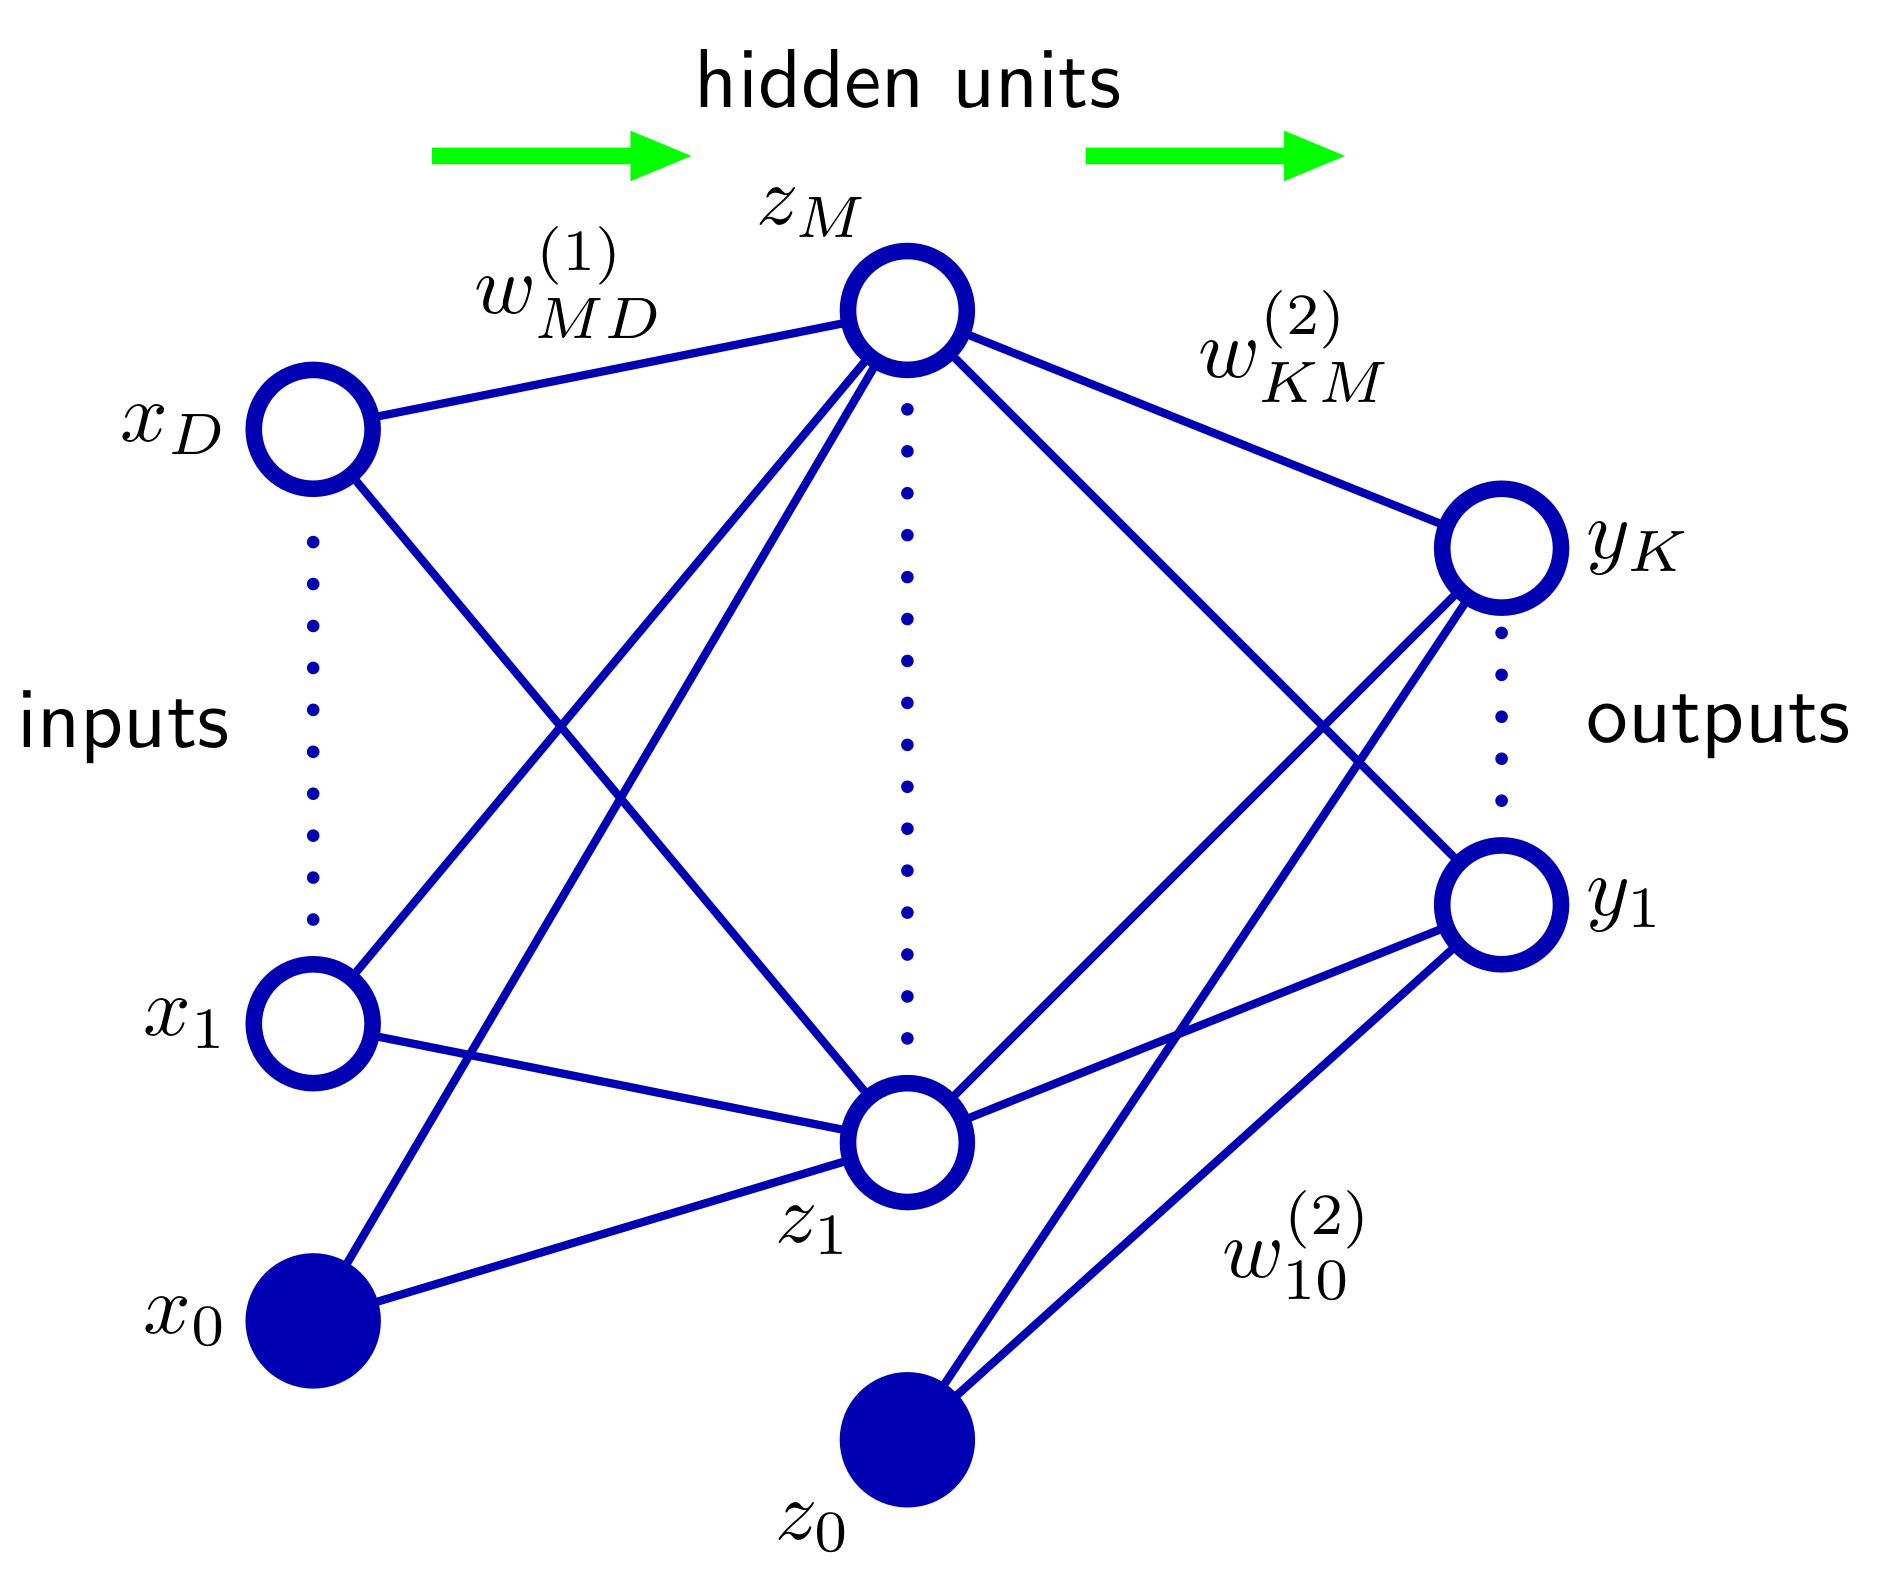
\includegraphics[width=0.5\textwidth]{files/figs/mlp.png}
 \caption{Feedforward neural network with two densely connected layers. Each line corresponds to one trainable parameter. $x_0$ and $z_0$ can be seen as ones added to the inputs introducing the bias terms \cite{Bishop2006}.}
 \label{fig:dense}
\end{figure}

\subsubsection{Convolutional layers}
Convolutional layers have proved successful for feature extraction from for instance time series or images. A reason for this is that they are equivariant to translation, meaning that patterns in a time series will be recognized in the same way no matter at which time steps they occur. The 1D convolution operation can be seen in \eqref{eq:conv}. When applied to for instance images it is performed in two dimensions.

\begin{equation}
 (x * w)(t) = \sum_{a=-\infty}^\infty x(a)w(t-a)
 \label{eq:conv}
\end{equation}

$x$ is the input and $w$ is the kernel or filter which consist of the trainable parameters. As the kernel size is not affected by the input size the convolutional layer can be applied to inputs of different size, which is not possible with for instance the fully connected layer \cite{Goodfellow2016}.

, layers, optimizers

\section{Training of }
% The training of a network is performed by evaluating a loss function, which describes the desired behavior, on the training data.

During training of a network a loss function, $\mathcal{L}$, which describes the desired behavior, is evaluated on the training data. To improve the performance of the model its parameters are changed to minimize this loss. In deep learning problems this optimization is usually performed with some gradient descent inspired method, shown in \eqref{eq:grad-desc}, where the parameters are updated in the direction which reduces the loss the most. With a large training data set the computation of the gradient quickly becomes expensive. A remedy for this has been to use stochastic or mini-batch gradient descent methods. Such algorithms use one or a few data points from the training set to estimate the gradient for each parameter update. Algorithms common today often use momentum, where previous gradients affect the parameter update direction, and adaptive learning rates (step size of parameter update), allowing different learning rate for different parameters \cite{Goodfellow2016}. One example of such a method is the Adam optimizer \cite{Kingma2015}.

\begin{equation}
 \pmb{W}_{k+1} = \pmb{W}_k - \alpha \pmb{D}
 \label{eq:grad-desc}
\end{equation}
\begin{conditions}
 $$\pmb{W}_k$$     & = & model parameters at iteration $k$ \\
 $$\alpha$$        & = & learning rate or step size \\
 $$\pmb{D}$$       & = & parameter update direction, e.g. $\frac{\partial \mathcal{L}}{\partial \pmb{W}}$ or a weighted average of earlier gradients
\end{conditions}

The gradients of the loss with respect to the model parameters are calculated using the back-propagation algorithm \cite{Rumelhart1987} which recursively uses the chain rule, \eqref{eq:chain}, to propagate the loss gradient through the network.

\begin{equation}
 \frac{dz}{dx} = \frac{dz}{dy}\frac{dy}{dx}
 \label{eq:chain}
\end{equation}

For a network where $f_0, f_1, \hdots, f_n$ denotes the outputs of the $n+1$ layers, with corresponding layer parameters $\pmb{w}_0, \pmb{w}_1, \hdots, \pmb{w}_n$ and loss function $\mathcal{L}$ the gradient is calculated by first performing a forward pass of input $\pmb{x}$. This allows for computation of the the gradient w.r.t. the output of the final layer, $f_n$, either analytically or using automatic differentiation. As both the structure and the parameters of the layers are known this can be used to calculate the gradient w.r.t. the parameters in that layer, $\pmb{w}_n$, as well as the output of the previous layer, $f_{n-1}$. By applying \eqref{eq:bp-layer} recursively the gradient is propagated through the network and from this \eqref{eq:bp-params} gives the gradients needed for the optimization.

\begin{subequations} \label{eq:backprop}
 \begin{align}
  \frac{\partial \mathcal{L}}{\partial f_k} & = \frac{\partial \mathcal{L}}{\partial f_{k+1}} \frac{\partial f_{k+1}}{\partial f_k} \label{eq:bp-layer} \\
  \frac{\partial \mathcal{L}}{\partial \pmb{w}_k} & = \frac{\partial \mathcal{L}}{\partial f_{k}} \frac{\partial f_{k}}{\partial \pmb{w}_k}    \label{eq:bp-params}
 \end{align}
\end{subequations}

\subsubsection{Loss functions}
For a classification problem with $K$ mutually exclusive classes the categorical cross-entropy is commonly used. With this loss the labels are one-hot encoded meaning that each label is represented by $K$ binary variables, i.e. $y_i \in \mathbb{Z}_2^K$. Each variable represents a class and $y_i^{(k)} = 1$ for the $k$ corresponding to the class of the label and 0 otherwise. The final layer of the model has $K$ outputs with softmax activation. The loss to be minimized is shown in \eqref{eq:cat-cross-entr} \cite{Bishop2006}.

\begin{equation}
 \mathcal{L}(\pmb{x}, \pmb{W}) = - \sum_{i=1}^N \sum_{k=1}^K \lambda^{(k)} y_i^{(k)} \log \hat{y}_i^{(k)}(x_i, \pmb{W})
 \label{eq:cat-cross-entr}
\end{equation}
\begin{conditions}
    $$y_i^{(k)}$$       & = & the correct binary label of class $k$ for data point $i$ in the training set \\
    $$\hat{y}_i^{(k)}$$ & = & the corresponding prediction from the model \\
    $$\lambda^{(k)}$$   & = & weight for class $k$.
\end{conditions}

The categorical cross-entropy will aim to maximize the predicted probability for the correct class. However, incorrect probabilities have no direct effect on the loss. To be able to affect what kind of errors the model makes in its predictions a modification of this loss can be used. This modified loss, here referred to as confusion-entropy, introduces a matrix, $U$, which can be seen as a target confusion matrix distribution. Entries in $U$ rewards predictions at the corresponding positions in the confusion matrix, including possible incorrect classifications.

skriv ekvation

skriv om att de har samma extrempunkt (ynk=1)



\subsubsection{activations osv, typ softmax, relu}



%The convolution, $(x * w)(t)$, can be seen as a weighted average of some points around $x(t)$

\section{Historical background of deep learning} \label{sec:dl-history}
In 1943 McCulloch and Pitts \cite{McCulloch1943} presented a mathematical model of a neuron which at the time had limited capabilities (e.g. it did not learn), but lay the foundations for much of what today is considered to be deep learning. Ivakhnenko and Lapa \cite{Ivakhnenko1965} introduced what would later be called deep learning with the first multi-layered network in 1965. The first convolutional network was introduced by Fukushima in 1980 \cite{Fukushima1980}. A few years later, in 1989, LeCun et al. \cite{LeCun1989} showed it possible to train such networks with backpropagation and illustrated their effectiveness for computer vision problems. In 2009 Raina et al. \cite{Raina2009} suggested that \glspl{dnn} could efficiently be trained on \glspl{gpu}. Krizhevsky et al. \cite{Krizhevsky2012} used this when they with AlexNet proved it possible to train deeper networks which also greatly outperformed models of the time at computer vision tasks. Since then deep learning based methods has been adopted in various fields, such as computer vision, natural language processing, and even autonomous vehicles \cite{NazmusSaadat2020}.

\section{Explainability} \label{sec:explainability}
Much of the recent progress in the deep learning space is inherently incomprehensible for us humans, due to its black-box nature and the size of the models \cite{Du2018}. However, explainability is important at many stages of the development of an AI-system. When the systems performance is at sub-human levels it simplifies for human experts to improve it. When the system achieves similar results human experts it can help enforce trust to the system. Finally, in a scenario where the AI outperforms humans it can help us get a better understanding of the problem \cite{Selvaraju2016}. With these methods playing a bigger role in fields such as healthcare the importance of explainable decisions also grows from a legal and ethical perspective \cite{Amann2020}.

\subsubsection{Gradient-weighted Class Activation Mapping (Grad-CAM)} \label{sec:grad-cam}
Although most deep learning models are not interpretable there are post-hoc methods which tries to explain decisions. Selvaraju et al. \cite{Selvaraju2016} suggested one such method, called \gls{grad-cam}, where an activation map is calculated which shows what parts of the data is important for the decisions. Considering a neural network with convolutional layers as feature extractors followed by \gls{gap} and dense layers for classification \gls{grad-cam} is based on the final part of the network. Let $y_c$ be the output corresponding to class $c$ and $A$ be the final feature map of height $H$, width $W$, and with $F$ filters. The \gls{grad-cam} activation, $M_{GC}$, is then calculated as follows:

\begin{align}
 \begin{split}
  w_k^c &= \frac{1}{H \times W} \sum_{i=1}^H \sum_{j=1}^W \frac{\partial y_c}{\partial A_{ij}^k} \\
  M_{GC} &= ReLU \big ( \sum_{k=1}^F w_k^c A^k \big)
  \label{eq:grad-cam}
 \end{split}
\end{align}

The resulting activation map is importance values $\in \mathbb{R}^{H \times W}$. If the input is a time series this means that by designing the network to not alter the time dimension an importance value is obtained for each time step.

\section{Consistent Rank Logits (CORAL)}
Categorical data with a natural ordering are considered to be ordinal, examples of such data are the response to some medical treatment (e.g. poor, fair, good) \cite{Agresti2007} or the age of a person \cite{Cao2019}.

When classifying ordinal data it is desirable to exploit the fact that the categories are ordered \cite{Agresti2007}. An ordinal classification problem, or ordinal regression as it is also referred to, can be formulated as assigning labels, $y \in \mathcal{Y} = \{\mathcal{C}_0, \mathcal{C}_1, \hdots, \mathcal{C}_{K-1} \}$, to inputs $\pmb{x}$, where the classes $\mathcal{C}_0 \prec \mathcal{C}_1 \prec \hdots \prec \mathcal{C}_{K-1}$ according to some ordering relation \cite{Cao2019}.

Li and Lin \cite{Li2007} presented a method for ordinal regression where the combined result of $K-1$ binary classifiers for $K$ classes were used. Each classifier checked whether the rank of the sample class was larger than rank $r_k \in \{r_1, \hdots r_{K-1}\}$. Niu et al. \cite{Niu2016} developed this further using a multi-output \gls{cnn} as $K-1$ binary classifiers, called OR-CNN. The classifiers share all weights except the ones in the output layer. This method achieved \gls{sota} performance on datasets where age was estimated based on facial images. However, consistency was not guaranteed in the predictions, e.g. sometimes simultaneously predicting an age under 20 and over 30. Cao et al. \cite{Cao2019} addressed this issue with \gls{coral} which is an architecture-agnostic method that can extend any neural network based classifier. Similarly to OR-CNN \gls{coral} uses $K-1$ binary classifiers, here however sharing all weights parameters apart from the biases in the output layer. Instead of representing the labels as one-hot encodings they are now formed as $K-1$ binary labels, i.e. $y \in \mathbb{Z}_2^{K-1}$, where $y_i^{(k)} = 1$ if the the rank of the class is greater than $r_k$ and 0 otherwise. By minimizing the loss function

\begin{equation}
 \mathcal{L}(\pmb{x}, \pmb{W}, \pmb{b}) = - \sum_{i=1}^N \sum_{k=1}^{K-1} \lambda^{(k)} [\log(\sigma(g(\pmb{x}_i, \pmb{W}) + b_k))y_i^{(k)} + \log(1 - \sigma(g(\pmb{x}_i, \pmb{W}) + b_k))(1 - y_i^{(k)})],
 \label{eq:coral-loss}
\end{equation}

\begin{conditions}
 $$\pmb{W}$$               & = & all model parameters except biases of final layer \\
 $$\pmb{b}$$               & = & bias weights of final layer \\
 $$\lambda^{(k)}$$         & = & loss weight for class $k$ \\
 $$g(\pmb{x}_i, \pmb{W})$$ & = & output of penultimate layer \\
 $$\sigma(z)$$             & = & logistic sigmoid function, $1/(1 + \exp(-z))$ \\
 $$\sigma(g(\pmb{x}_i, \pmb{W}) + b_k)$$ & = & predicted output of binary classifier $k$
\end{conditions}

it can be shown that

\begin{equation}
 b_1 \geq b_2 \geq \hdots \geq b_{K-1}.
\end{equation}

The proof can be found in \cite{Cao2019} and from this and the shared weights it follows that

\begin{equation}
 \widehat{P} \big( y_i > r_1 \big) \geq \widehat{P} \big( y_i > r_2 \big) \geq \hdots \geq \widehat{P} \big( y_i > r_{K-1} \big)
\end{equation}

since the only thing that differs between the predictions is the bias. The probabilities for the individual classes are computed from this as

\begin{equation}
 \begin{alignedat}{2}
  &\widehat{P}\big(\mathcal{C}_0 \big) &&= 1 - \widehat{P}\big(y_i > r_1\big) \\
  &\widehat{P}\big(\mathcal{C}_1 \big) &&= \widehat{P}\big(y_i > r_1\big) - \widehat{P}\big(y_i > r_2\big) \\
  & &&\vdots \\
  &\widehat{P}\big(\mathcal{C}_{K-1} \big) &&= \widehat{P}\big(y_i > r_{K-1}\big).
 \end{alignedat}
\end{equation}

% !TEX root=../../mt-motion-analysis.tex
\chapter{Related work - Human Pose Estimation} \label{sec:pose_estimation}
\gls{hpe} is a well explored problem which, like many other computer vision tasks has developed rapidly in the recent years. The reasons behind this progress can mainly be explained by two factors. Firstly the emergence of computing power discussed in Section \ref{sec:ML}, allowing more powerful deep learning models. Secondly several datasets with images labeled with human body joints has been made available \cite{Chen2020}. These datasets not only provide data, but also introduces competition in the research community making it possible to compare the results of different approaches.

\section{Datasets} \label{sec:datasets}
Some of the widely used datasets today are \gls{mpii} \cite{Andriluka2014}, \gls{coco} \cite{Lin2014}, \gls{aic-hkd} \cite{Wu2017}, and \gls{coco-whole} \cite{Jin2020}.% The two COCO datasets will now be described in more detail.

The \gls{coco} dataset consists of 328k images containing 91 different object types. The images come from Google, Bing, and Flickr image search and are mainly hand annotated through Amazon  Mechanical Turk. The interesting part of the dataset for this work is the one with human poses. In total there are 250k instances of people labeled with joint locations \cite{Lin2014}. The joints, 17 per person, in the dataset can be seen in Figure \ref{fig:coco}. Along with the datasets containing body keypoints mentioned above there are also datasets with dense keypoints for specific bodyparts, e.g. OneHand10k \cite{Wang2019}. \gls{coco-whole} is an attempt to combine these two types of datasets by extending \gls{coco} with dense keypoints at hands, feet, and faces. The resulting 133 joints can be seen in Figure \ref{fig:coco-wholebody}.

\begin{figure}
 \centering
 \begin{subfigure}[t]{0.4\textwidth}
  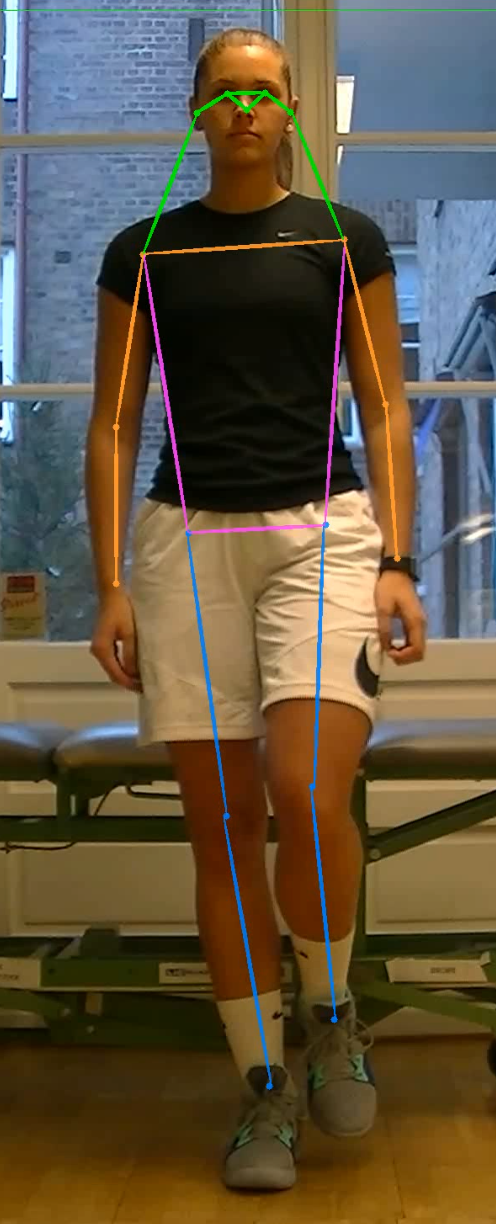
\includegraphics[width=\textwidth]{files/figs/coco.png}
  \caption{Regular \gls{coco}.}
  \label{fig:coco}
 \end{subfigure}
 ~
 \begin{subfigure}[t]{0.4\textwidth}
  \includegraphics[width=\textwidth]{files/figs/coco-whole.png}
  \caption{\gls{coco-whole}.}
  \label{fig:coco-wholebody}
 \end{subfigure}
 \caption{Keypoints for the two COCO datasets.}
\end{figure}


% \section{Pose estimation models}
\section{Background - Human pose estimation}
The \gls{hpe} problem has been explored since long before the most recent deep learning era. Pictoral Structures were introduced by Fishler and Elschlager in the 1970s. This meant identifying individual parts or features in images modeled with pair-wise spring-like connections \cite{Fischler1973}. After the success of deep learning described in Section \ref{sec:dl-history} Toshev and Szegedy \cite{Toshev2014} presented DeepPose, the first \gls{hpe} method based on \glspl{dnn}. Today's \gls{hpe} methods are generally categorized as top-down or bottom-up approaches. This has to do with how they handle multiple persons. Bottom-up models starts by finding all keypoints for all persons in an image and then match them together to form persons. Top-down models on the other hand starts by finding bounding boxes for all individuals and then identifies keypoints for one person at a time. The sequential nature of the top-down methods and the fact that two models are needed means that bottom-up models scale better with the number of persons to analyze. However top-down models tends to be more accurate \cite{Cheng2019}.
% Since the application we present requires single person recognition only the top-down \gls{sota} methods presented below are used.

\section{Pose estimation models}
Below the \gls{hpe} models used in our work are presented. As we are interested in single person recognition the model used is of top-down type.

\subsection{High-Resolution Net (HRNet)} \label{sec:hrnet}
Sun et al. \cite{Sun2019} presented the \gls{hrnet} architecture in 2019, initially for \gls{hpe}, but also for other computer vision tasks such as semantic segmentation and object detection. Such problems had traditionally been solved using networks built on high-to-low resolution convolutions with increasing numbers of feature maps (e.g ResNet \cite{He2016}, VGGNet \cite{Simonyan2015}). The classification task was solved in the low-resolution space and then transformed back to form the high-resolution representation needed for e.g. the \gls{hpe}. Sun et al's proposed architecture preserves a high resolution representation throughout the network. It does so while also producing low-resolution/high dimensional representations suitable for classification.

The network architecture is shown in Figure \ref{fig:hrnet} and consists of four stages (blue blocks in depth direction in Figure) with convolutional layers. After each stage a new low-resolution representation is created by performing strided convolutions. At these instances the existing representations also exchange information by either nearest neighbor upsampling or strided convolutions. The $K$ estimated keypoints are represented as heatmaps, $\{\mathbf{H}_1, \hdots, \mathbf{H}_K\}$, indicating the locations. These heatmaps are formed from the last high-resolution feature map (top right in Figure \ref{fig:hrnet}). Corresponding ground truth heatmaps are generated by applying 2D Gaussians to the correct keypoint locations and the model is trained by minimizing the mean squared error between these \cite{Sun2019}. Although a high resolution heatmap is desirable as it gives smaller quantization errors, the computational cost increases quadratically with the size \cite{Zhang2020}. Hence, to make the computations feasible the input image is downsampled through strided convolutions, resulting in a four times smaller heatmap \cite{Wang2020}.  %The heatmaps used for training are generated by applying 2D Gaussians to the dataset keypoints.

\begin{figure}
 \centering
 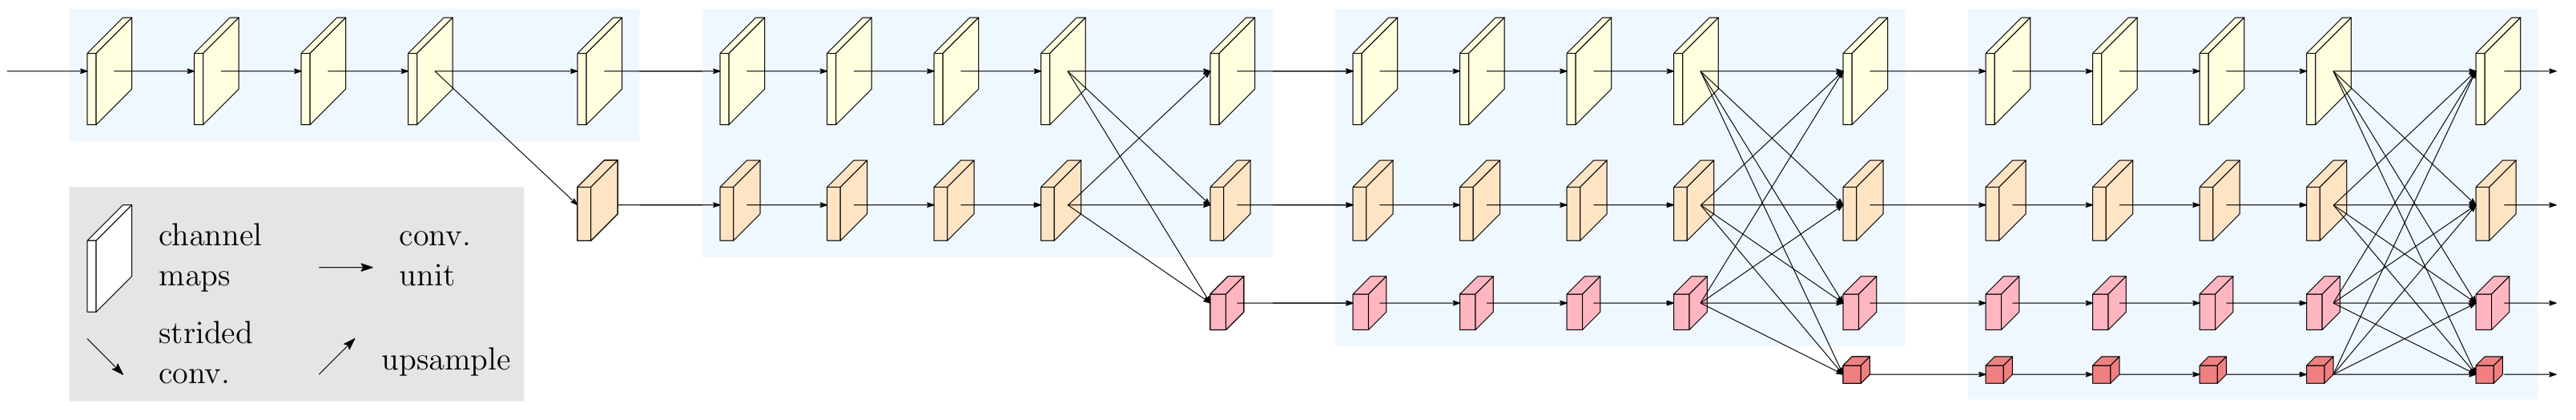
\includegraphics[width=\textwidth]{files/figs/hrnet.png}
 \caption{Network architecture for \gls{hrnet}. The top row shows high resolution representations with fewer number of feature maps. Each step downwards reduces the resolution with a factor of two while the number of feature maps are doubled \cite{Wang2020}.}
 \label{fig:hrnet}
\end{figure}

\subsection{Distribution-Aware coordinate Representation of Key-point (DARK)} \label{sec:dark}
As discussed above a high resolution heatmap should result in higher accuracy, but is computationally expensive. Zhang et al. \cite{Zhang2020} propose a way to reduce the quantization error by i) analyzing the distributions of the predicted heatmaps, and ii) creating the training heatmaps in a slightly new fashion.

The actual keypoint location is found at the maximal activation of the heatmap. Since it is smaller than the actual image this turns into a sub-pixel localisation problem. Newel et al. \cite{Newell2016} empirically found that a weighted average between the two highest activations, according to \eqref{eq:pixel-empiric}, yielded a good result.

\begin{equation}
  \pmb{p} = \symbfit{m} + \frac{1}{4}\frac{\symbfit{s} - \symbfit{m}}{\lVert \symbfit{s} - \symbfit{m} \rVert_2}
  \label{eq:pixel-empiric}
\end{equation}
\begin{conditions}
    \italbf{p}   & =   & predicted maximum \\
    \italbf{m}      & =   & highest activation \\
    \italbf{s}      & =   & second highest activation
\end{conditions}

This has been the de facto standard heatmap decoding, but Zhang et al. suggests using the fact that the heatmaps used for training usually are created as 2D Gaussian distributions, i.e. that the heatmaps can be expressed as \eqref{eq:gaussian-heatmap}.

\begin{equation}
  \mathcal{G}(\pmb{x}; \pmb{\mu}, \Sigma) = \frac{1}{2\pi \mid \Sigma \mid^{\frac{1}{2}}}
  \exp \Big( -\frac{1}{2} (\pmb{x} - \pmb{\mu})^\intercal \Sigma^{-1} (\pmb{x} - \pmb{\mu}) \Big)
  \label{eq:gaussian-heatmap}
\end{equation}
\begin{conditions}
    $$\pmb{\mu}$$ & =   & maximum of heatmap \\
    \italbf{x}    & =   & pixel location \\
    $$\Sigma$$    & =   & diagonal covariance matrix
\end{conditions}

By Taylor expanding of the logarithm of \eqref{eq:gaussian-heatmap} in the point \italbf{m}, i.e. the point with the highest sampled activation, an expression for $\pmb{\mu}}$ is obtained:

\begin{equation}
    \pmb{\mu} = \pmb{m} - \Big(\mathcal{D''}(\pmb{m})\Big)^{-1} \mathcal{D'}(\pmb{m})
    \label{eq:opt-mu}
\end{equation}
\begin{conditions}
    $$\mathcal{D}(\pmb{x})$$ & = & $-\frac{1}{2} (\pmb{x} - \pmb{\mu})^\intercal \Sigma^{-1} (\pmb{x} - \pmb{\mu})$, \\
      & & i.e. the non constant term in the logarithm of $$\mathcal{G}$$ \eqref{eq:gaussian-heatmap}
\end{conditions}

The derivatives $\mathcal{D'}(\pmb{m})$ and $\mathcal{D''}(\pmb{m})$ are efficiently estimated from the heatmap. As this approach strongly assumes a Gaussian structure it is proposed to modulate the heatmap before estimating the maximal activation. This is done by performing a convolution with a Gaussian kernel with the same covariance as the one used for the training data.

The second improvement suggested by Zhang et al. concerns the creation of the training heatmaps. Traditionally these have been created from the quantized keypoint locations, resulting in a slightly biased heatmap. In Figure \ref{fig:pixel-quantization} this would correspond to having the peak activation in the purple dot. By instead using the non-quantized location an unbiased heatmap is obtained. This would correspond to having the peak off-grid, in the blue dot in Figure \ref{fig:pixel-quantization}.

\begin{figure}
  \centering
  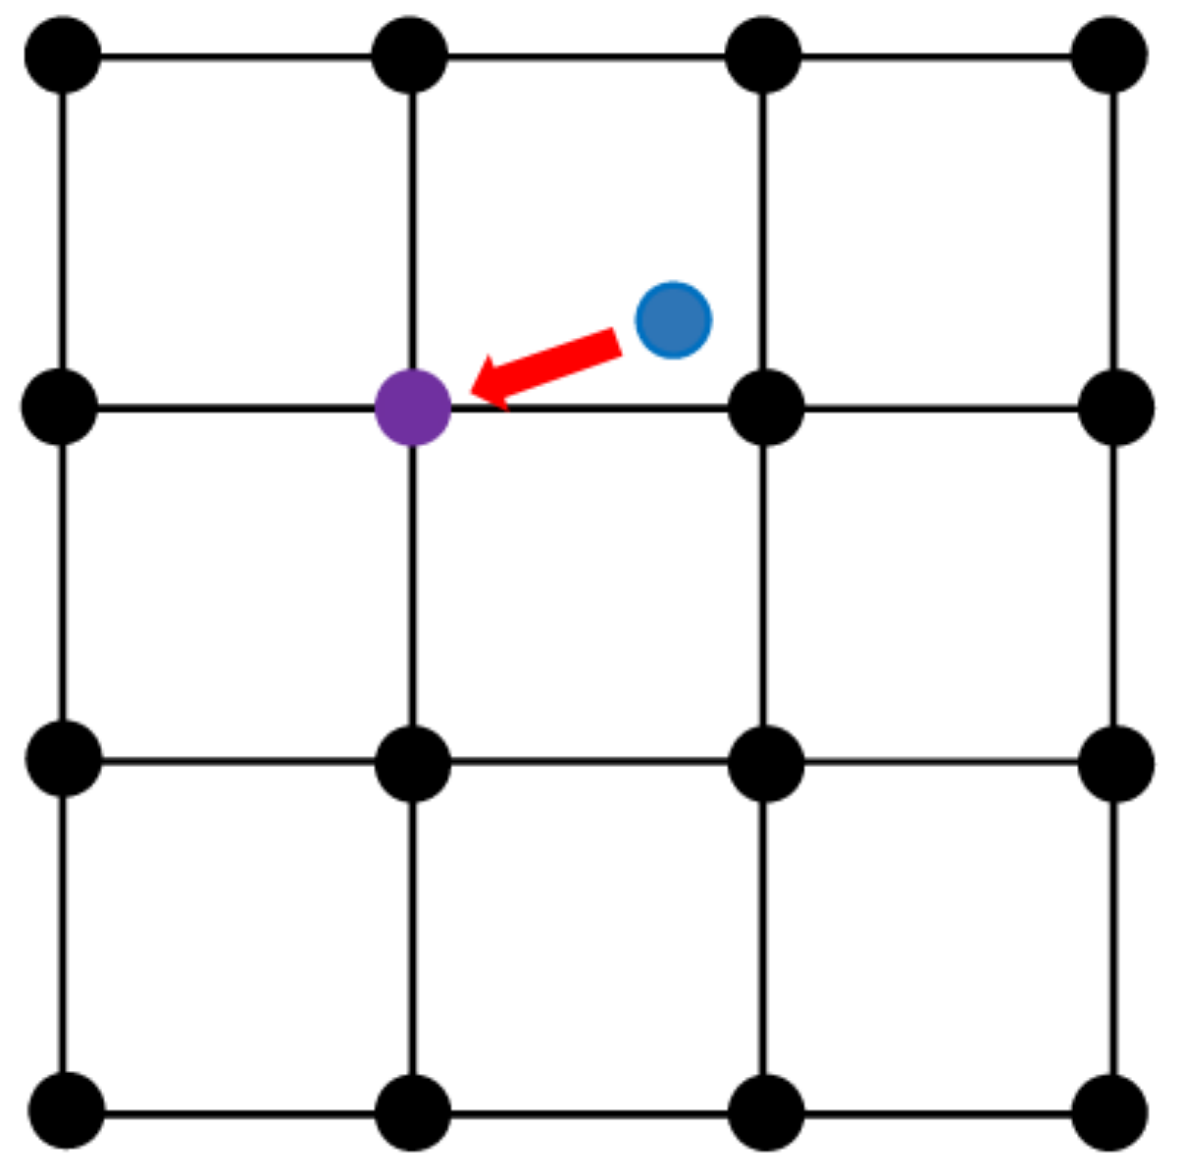
\includegraphics[width=0.4\textwidth]{files/figs/quantization.png}
  \caption{Quantization error due to off-grid keypoint location. Correct location (blue) represented by on-grid coordinate, here using floor quantization \cite{Zhang2020}. SKRIV ANTAGLIGEN NAGOT BATTRE HAR!!!!!}
  \label{fig:pixel-quantization}
\end{figure}

% The combination of DARK and HRNet is the method that as of today yields the highest accuracy on both the COCO and MPII dataset

% !TEX root=../../mt-motion-analysis.tex
\chapter{Related work - Time Series Classification} \label{sec:tsc}
\section{Background - Time series classification}
Time series are sequences of data ordered in time [H'R KANSKE TA EN FIN DEFINITION FR[N ANDREAS...].

SKA JAG HA DESSA DEFINITIONER? HANVISAR JAG TILL DEM NGNSTANS?

\begin{definition}
  \text{A univariate time series of length n, with ordered indices}
  $$X = \left[x_1, x_2, \hdots, x_n\right]^\intercal$$
  \label{def:uts}
\end{definition}

\begin{definition}
    \text{A multivariate time series of length n, with M channels}
    $$\pmb{X} = \left[X_1, \hdots, X_M\right]$$
\end{definition}

The \gls{tsc} task is about finding a function, $f: \mathbb{R}^{n \times M} \rightarrow \mathbb{R}$, that assigns one label to each, possibly multivariate, time series. The problem bares strong resemblance with that of image classification, but with the two spatial dimensions replaced by one temporal dimension. Despite this the use of end-to-end deep learning models is not as dominant in the \gls{tsc} community \cite{IsmailFawaz2019}. Similarily to the fields of computer vision various datasets has emerged recently. This has been important for the development of \gls{tsc} as it allows for fair comparison between methods. One of the most widely used dataset collections today is the \gls{ucr} archive \cite{Dau2018} containing 85 different time series datasets.

Traditionally a nearest neighbor method together with dynamic time warping has been used for classification \cite{Bagnall2017}. Simply put, this means that a time series during classification is compared to the training data and assigned the class of the most similar time series. Lines and Bagnall suggested a method where an ensemble of 11 nearest neighbor classifiers with different similarity measures \cite{Lines2015} yielded \gls{sota} results. Bagnall et al. \cite{Bagnall2015} developed the idea of ensemble based classifiers with \gls{cote}, where 35 different classifiers using different transforms was used. Lines et al. \cite{Lines2016} extended \gls{cote} further with two new classifiers resulting in \gls{hive-cote}. One drawback with \gls{hive-cote} is the computational intensity, both during training and test time. Training time is large partly due to one of the transforms used is the Shapelet Transform with a time complexity of $O(n^2l^4)$, $n$ being the number of time series and $l$ the length of them. Due to the nature of the nearest neighbor algorithm the result of the 37 classifiers during test time needs to be compared to the corresponding result for each time series in the training set, yielding this method impractical for real-time use \cite{IsmailFawaz2019}.

In 2016 Zheng et al. \cite{Zheng2016} presented a neural network model based on convolutional layers for the classification task. Wang et al. \cite{Wang2017} developed these ideas and presented models with performance close to that of \gls{cote} on the \gls{ucr} archive. The development of neural network based classification has since then continued and below the two architectures inspiring our model are presented.

\section{Deep learning architectures}
The last few years the number of proposed neural network based time series classifiers has increased drastically. Below the two most influential architectures for our work are presented.

\subsection{InceptionTime} \label{sec:inception-time}
InceptionTime, presented by Fawaz et al. \cite{IsmailFawaz2020}, is, as the name suggests, inspired by Inception \cite{Szegedy2015} which is an architecture successful in computer vision tasks. It is comprised of several stacked Inception modules consisting of differently sized convolutions as well as pooling layers. To reduce the number of parameters in the network 1$\times$1 convolutions are often used as a dimensionality reduction. One such module can be seen in Figure \ref{fig:inception-module}. The architecture of Fawaz et al. is similar, but with only one temporal dimension instead of two spatial dimensions. As with the computer vision task the dimensionality is reduced, here through a bottleneck of size $m$. The bottleneck is achieved by convolutions with $m$ filters of length 1. The InceptionTime module is shown in Figure \ref{fig:inceptiontime-module}.

Figure \ref{fig:inceptiontime} shows how stacked modules makes up the InceptionTime architecture. Residual connections are used to decrease the risk of vanishing gradients once the network becomes deeper, as suggested by He et al. \cite{He2016}. The InceptionTime modules are followed by a \gls{gap} layer which averages each time series over its time dimension. The classification is performed by fully connected layers with softmax activations.

Many deep learning based time series classifiers experiences a significant variance in their accuracy, especially when evaluated on the \gls{ucr} archive with rather small training sets \cite{IsmailFawaz2019ensemble}. To overcome this Fawaz et al. suggest the use of an ensemble of identical InceptionTime networks, but with randomly initialized weights before training. The ensemble's output is then calculated as the average of the outputs of the individual models. Such an ensemble of five models achieves a performance similar to that of \gls{hive-cote} on the \gls{ucr} archive.
% As was showed with ResNet \cite{He2016} residual connections reduces the risk for vanishing gradients and enables deeper networks. Hence this is

% Using residual connections between blocks reduces the risk of vanishing gradients and allows for deeper networks

%The 1D convolutions together with dimensionality reduction allows for longer filters than what is feasible to use for images.

\begin{figure}
  \centering
  \begin{subfigure}[c]{0.6\textwidth}
    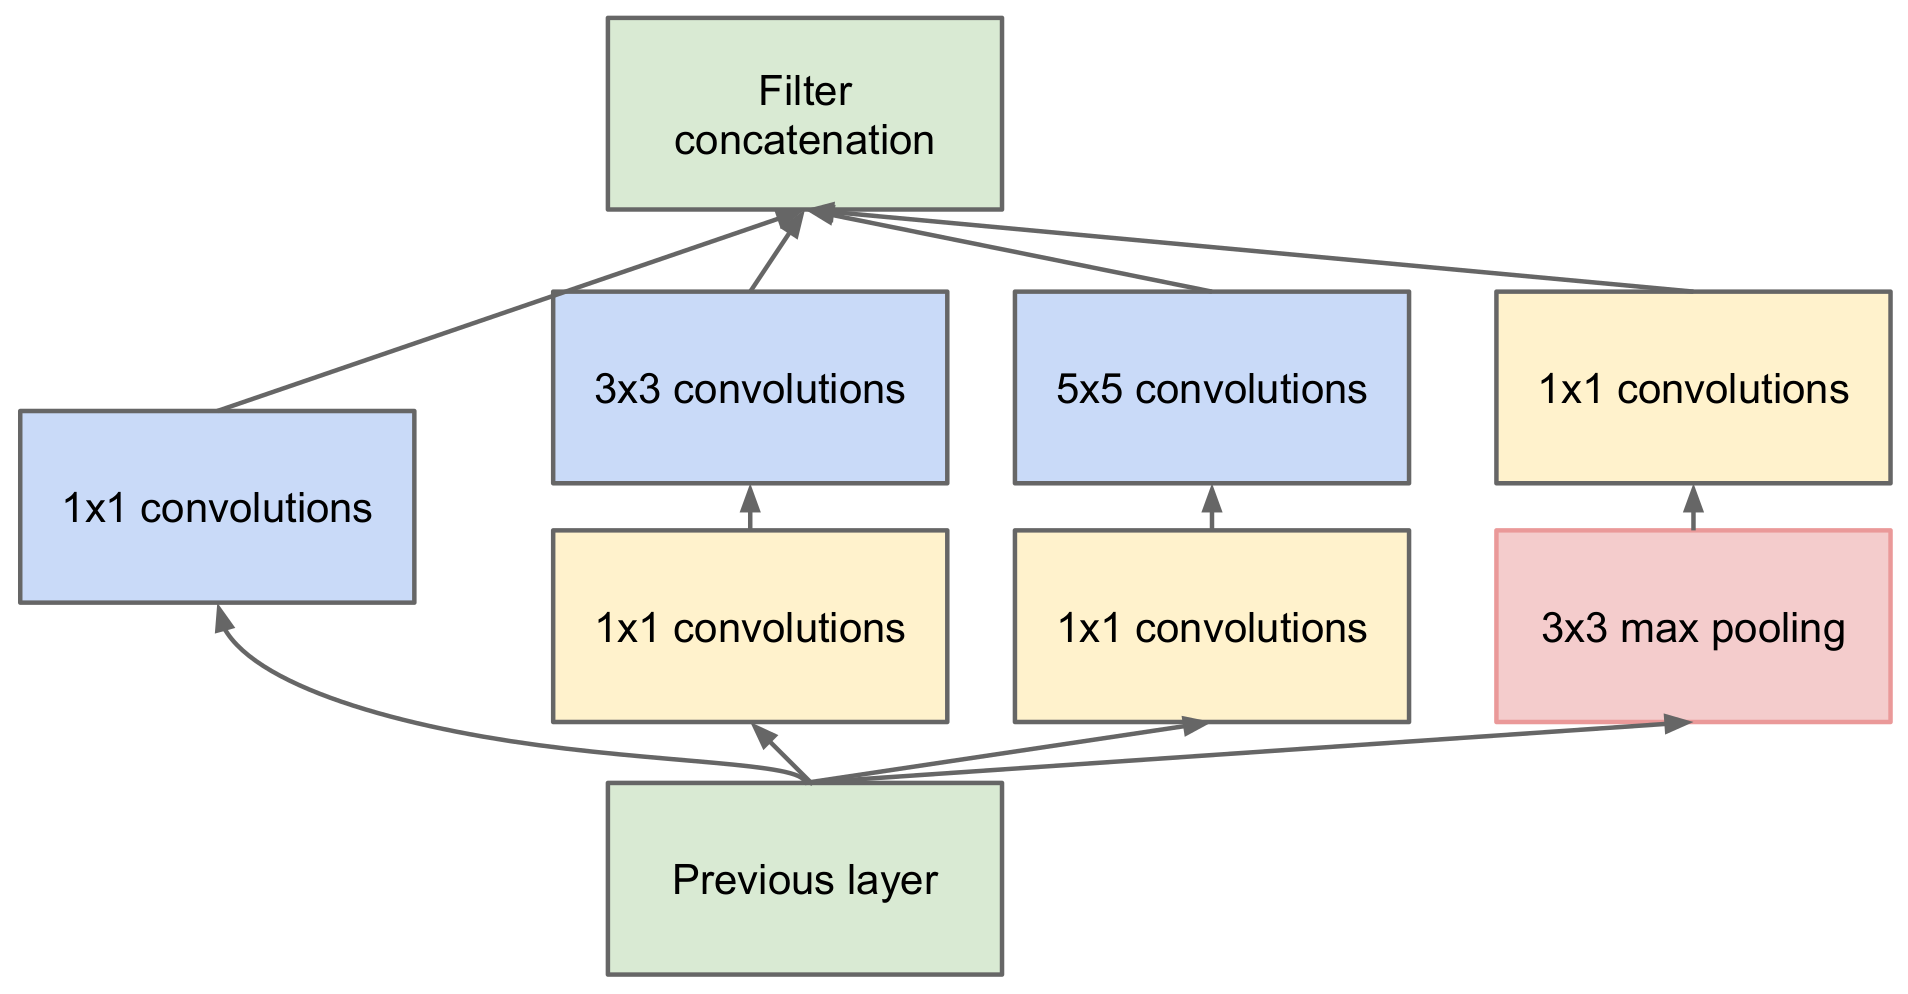
\includegraphics[width=\textwidth]{files/figs/inception-module-dimred.png}
    \caption{}
    % \caption{Inception module for computer vision \cite{Szegedy2015}.}
    \label{fig:inception-module}
  \end{subfigure}
  \begin{subfigure}[c]{0.6\textwidth}
    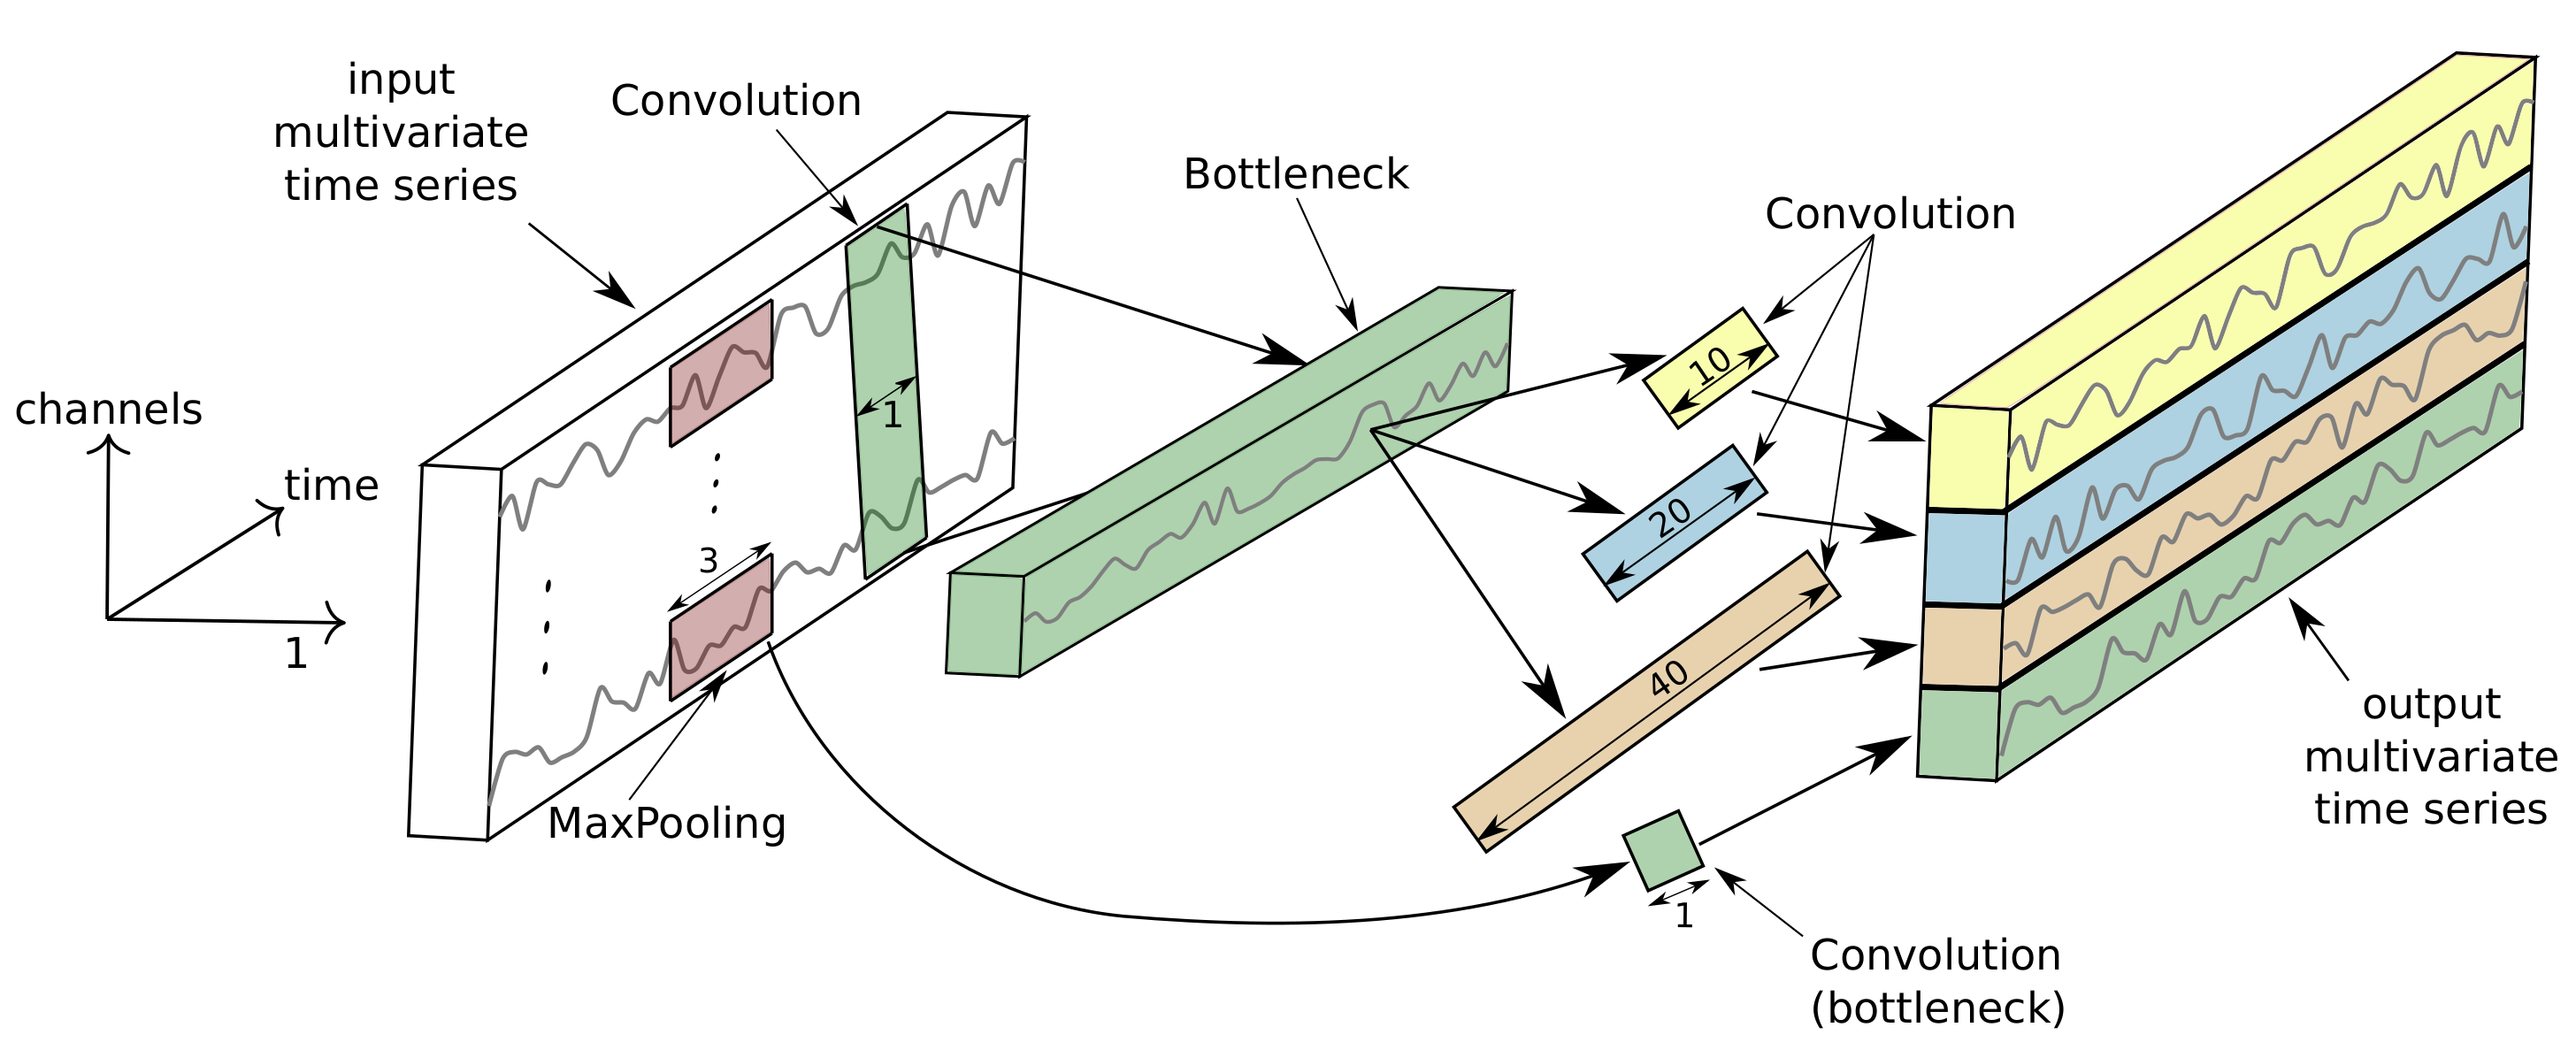
\includegraphics[width=\textwidth]{files/figs/inception-time-module.png}
    \caption{}
    % \caption{Inception module for \gls{tsc} \cite{IsmailFawaz2020}.}
    \label{fig:inceptiontime-module}
  \end{subfigure}
  \caption{Inception modules for computer vision (a) with dimensionality reduction ahead of the 3$\times$3 and 5$\times$5 convolutions and InceptionTime module for TSC (b), here illustrated with a bottleneck size of 1. Figures from \cite{Szegedy2015} and \cite{IsmailFawaz2020} respectively.}
\end{figure}

\begin{figure}
  \centering
  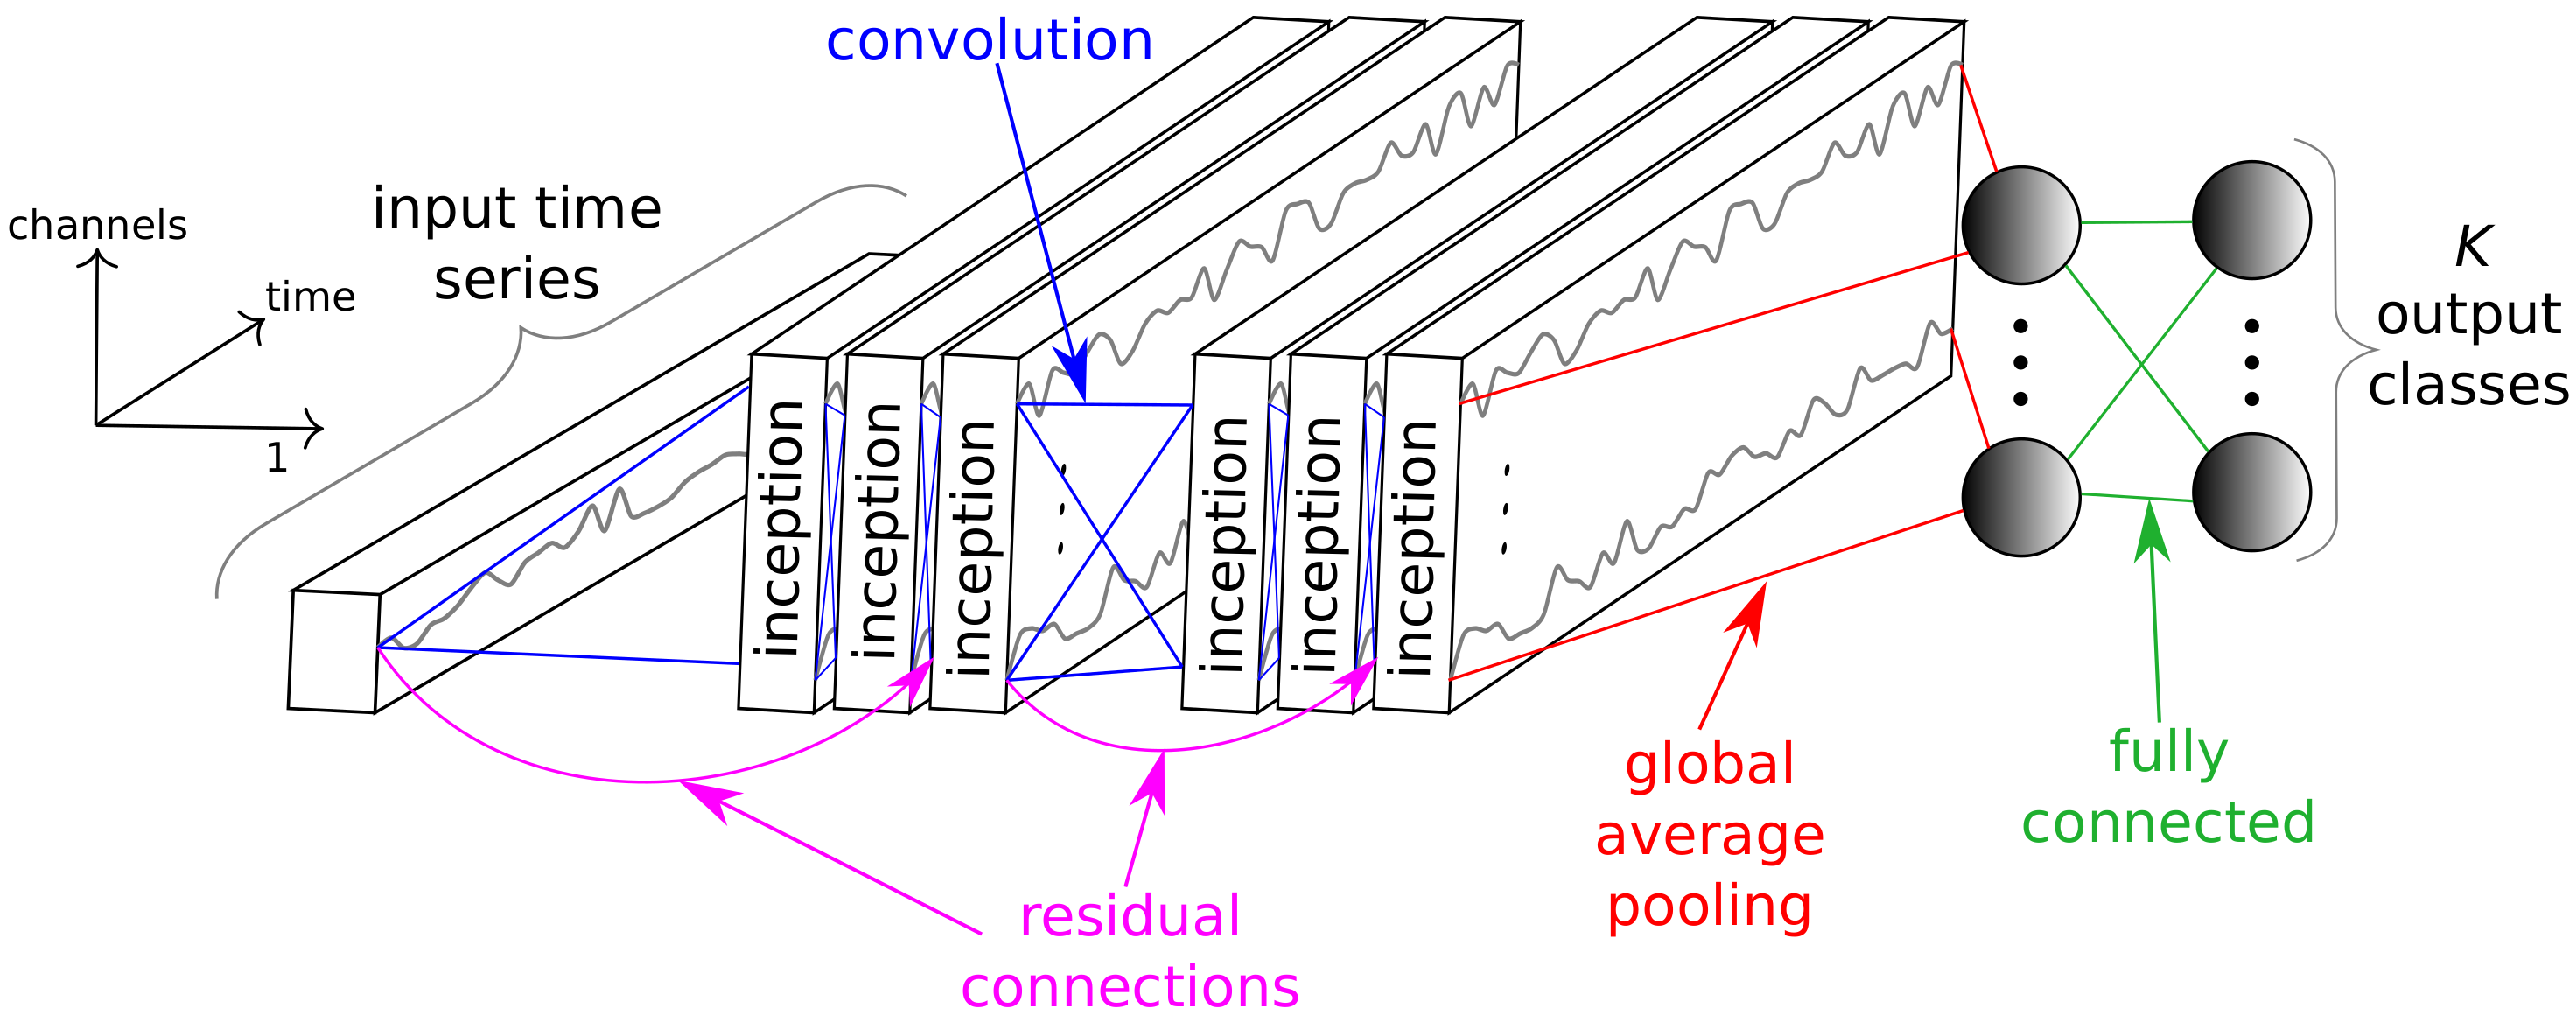
\includegraphics[width=0.6\textwidth]{files/figs/inceptiontime.png}
  \caption{InceptionTime architecture for TSC \cite{IsmailFawaz2020}.}
  \label{fig:inceptiontime}
\end{figure}

\FloatBarrier

\subsection{Explainable Convolutional Neural Network for Multivariate Time Series Classification (XCM)} \label{sec:XCM}
As discussed in Section \ref{sec:explainability} explainability is desirable, but not inherent in most black-box deep learning models. Fauvel et al. \cite{Fauvel2020} propose an architecture, \gls{xcm}, which allows for tracking which time steps and which inputs are important for the classification decision. By using 2D convolutions with kernels of size $ks$$\times$1, where $ks$ is the kernel size hyperparameter, the convolution is only performed in the time dimension and the input channels are kept separated throughout the feature extraction. Through dimensionality reduction from a 1$\times$1 2D convolution a single feature map for each input is produced. From this the importance of input channels and time steps can be traced using \gls{grad-cam}, described in Section \ref{sec:grad-cam}. In parallel to the channel specific features Fauvel et al. also suggests using 1D convolutions over all channels resulting in a combined feature map along the time dimension. The \gls{xcm} architecture is depicted in Figure \ref{fig:xcm}.

\begin{figure}
  \centering
  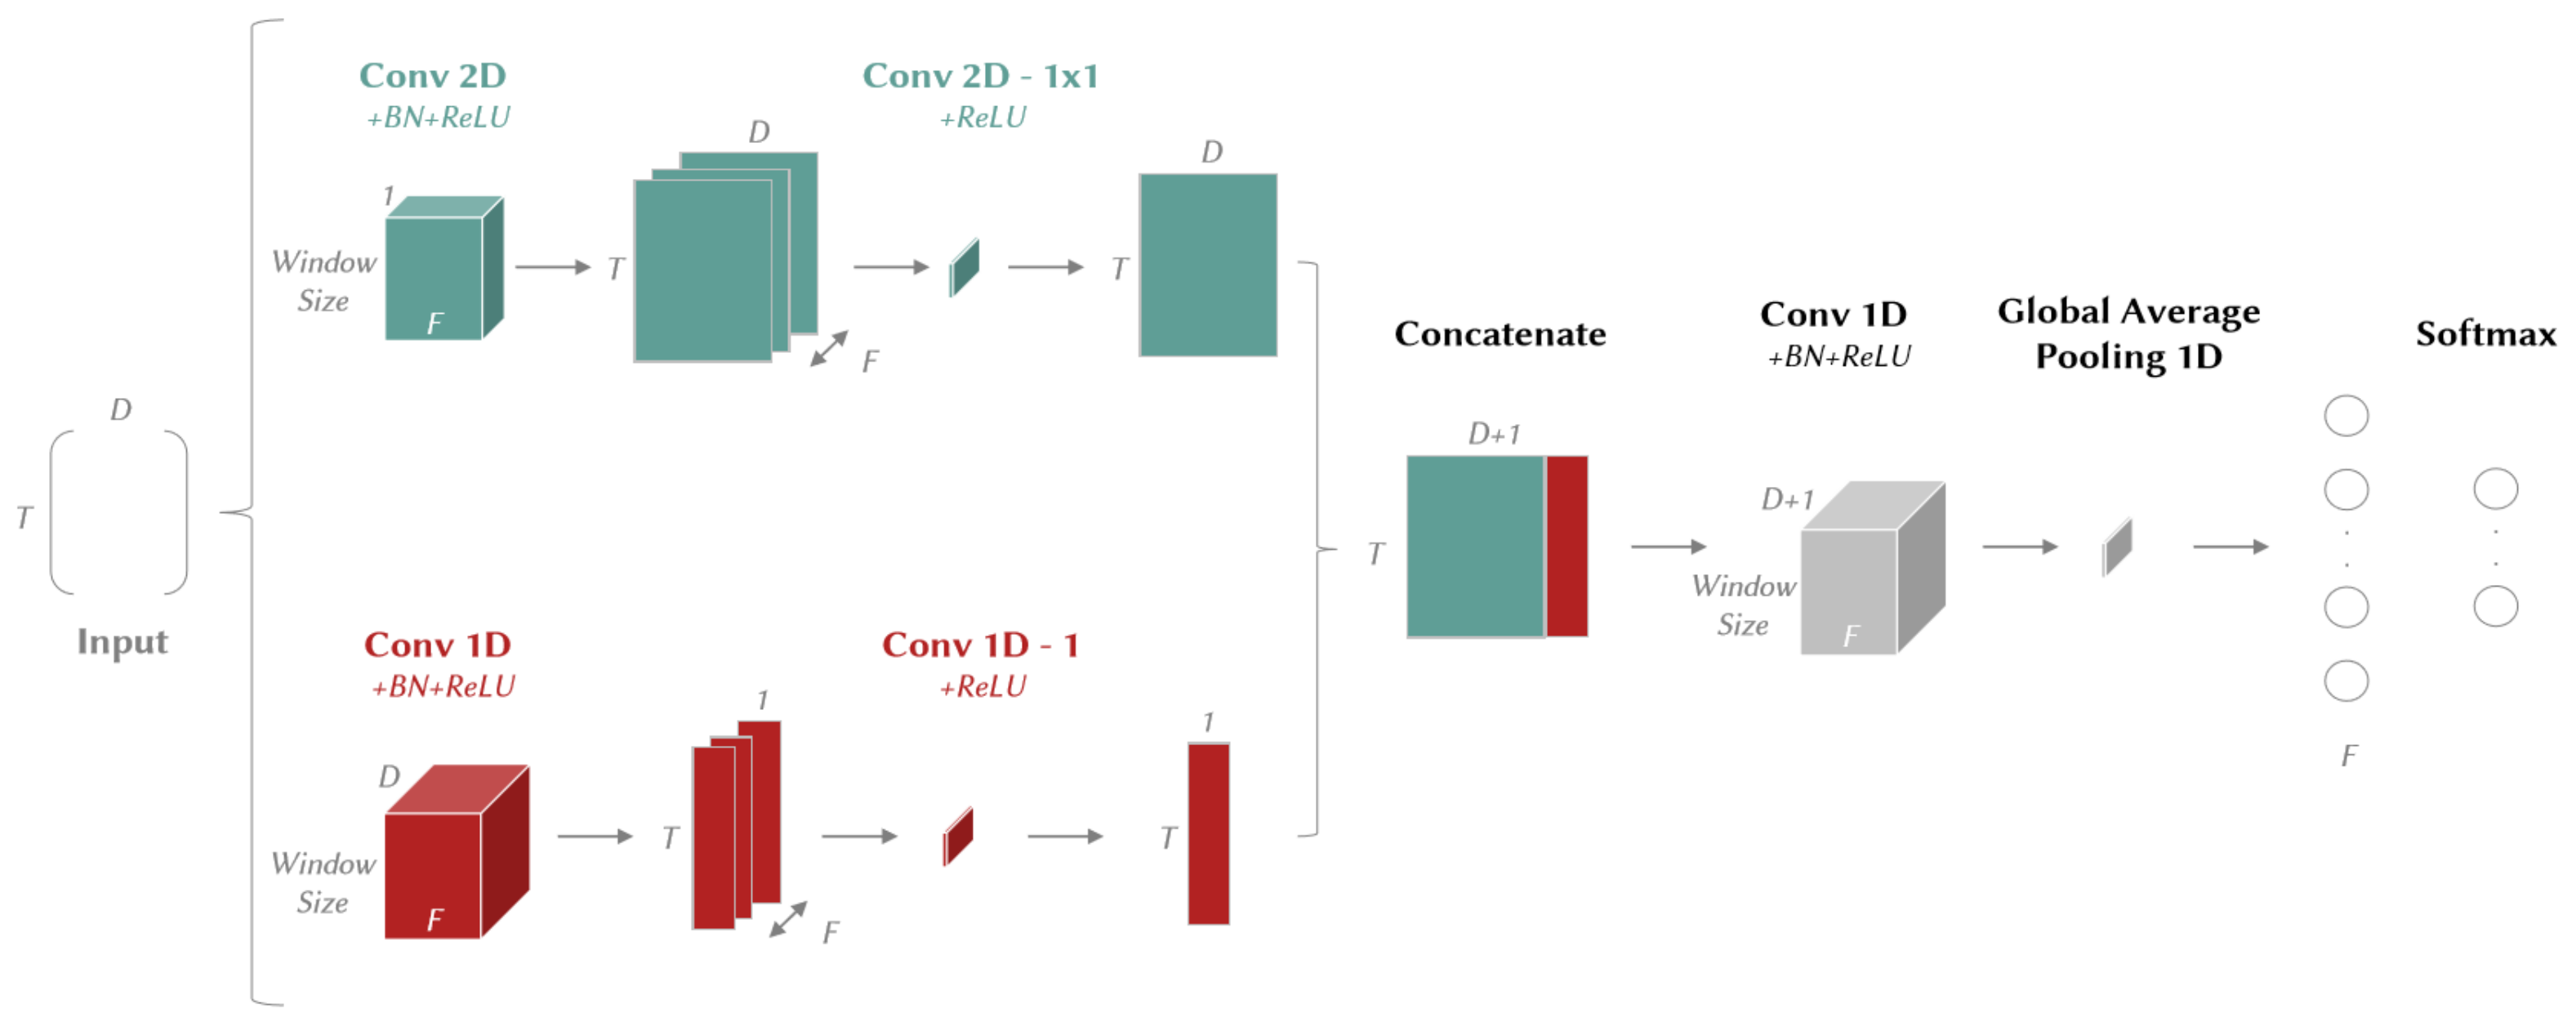
\includegraphics[width=0.7\textwidth]{files/figs/xcm.png}
  \caption{The XCM architecture with $BN$ - Batch Normalization, $D$ - number of input channels, $F$ - number of filters, $T$ - length of time series \cite{Fauvel2020}.}
  \label{fig:xcm}
\end{figure}

\FloatBarrier

% !TEX root=../../mt-motion-analysis.tex
%!TeX spellcheck = en-US
\chapter{Methods}
\section{Overview}
In this chapter the system for assessing POEs will be presented. This system is naturally divided into two parts where firstly the videos are analyzed. The first subsystem extracts body part coordinates of the subjects. This information is then passed to the second subsystem where it is used to calculate a score according to \cite{Nae2017}. The data is presented in Section \ref{sec:met-data} and the two subsystems are described in Sections \ref{sec:met-loc} and \ref{sec:met-class} respectively.

\section{Data}\label{sec:met-data}
The data available is in the form of videos each containing one subject, recorded from the front, performing three-five repetitions of specific motions. The motions are \textit{Single-leg squat, Forward lunge, Stair descending, Forward lunge, Single leg hop for distance, and Side hop}. Each motion has a number of POE scores associated with them. The motion-POE combinations are shown in Table \ref{tab:met:motion-poes}. In Sections \ref{sec:met-SLS}-\ref{} the motions and POEs evaluated in this project are described.

% The videos were recorded with different orientations and frame rates.
%
% The available videos has been assessed by a physiotherapist and for each repetition in each motion a number of POE scores has been awarded.


% \begin{table}
%  \centering
%  \caption{Motion-POE combinations available in the data.}
%  \label{tab:met:motion-poes}
%
%  \begin{tabular}{|c|ccccc|}
%   \hline
%   \backslashbox{POE}{Motion}                      &
%   \multicolumn{1}{c}{\begin{tabular}[c]{@{}c@{}}Single\\ leg squat\end{tabular}}   &
%   \multicolumn{1}{c}{\begin{tabular}[c]{@{}c@{}}Stair\\ descending\end{tabular}}   &
%   \multicolumn{1}{c}{\begin{tabular}[c]{@{}c@{}}Forward\\ lunge\end{tabular}}   &
%   \multicolumn{1}{c}{\begin{tabular}[c]{@{}c@{}}Single leg hop\\ for distance\end{tabular}}   &
%   \multicolumn{1}{c|}{\begin{tabular}[c]{@{}c@{}}Side\\ hop\end{tabular}}                      \\ \hline \hline
%
%   Trunk                                           & x & x &   & x & x \\ \hdashline
%   Hip                                             & x & x & x & x & x \\ \hdashline
%   \multicolumn{1}{|c|}{\begin{tabular}[c]{@{}c@{}}Femoral\\ valgus\end{tabular}} &
%   x                                               & x & x & x & x     \\ \hdashline
%   \multicolumn{1}{|c|}{\begin{tabular}[c]{@{}c@{}}Knee medial to\\ foot position\end{tabular}} &
%   x                                               & x & x & x & x     \\ \hdashline
%   \multicolumn{1}{|c|}{\begin{tabular}[c]{@{}c@{}}Femur medial\\ to shank\end{tabular}} &
%   x                                               & x & x & x & x     \\ \hdashline
%   Foot                                            & x &   &   &   &   \\ \hline
%  \end{tabular}
% \end{table}

bara skriva om sls? om det bara 'r sls jag bed;mt.. ocks[ skriva det som avgr'nsningar

\subsection{Single-leg squat, SLS} \label{sec:met-SLS}
The subject performed a squat standing on one leg to a knee angle of approximately $60\degree$. The exercise was repeated five times and the entire movement was used to assess the POEs \cite{Nae2020}. An illustration is shown in Figure \ref{}.

\subsection{Stair descending, SD}
The subject stepped down from a 30 cm step board. The exercise was repeated five times and POEs were evaluated for the loaded leg during loading phase \cite{Nae2020}. An illustration is shown in Figure \ref{}.

\subsection{Forward Lunge, FL}

Helo I am now mispealing.



% The data the system is designed for is in the form of videos each containing around five repetitions of some specific motion. For each repetition in each motion up to five POEs has been graded according to \cite{Nae2017}.


\section{Body part localization} \label{sec:met-loc}
% \subsection{Preprocessing}
% ...
% rotation, flip etc
% \subsection{Pose estimation}
%The pose estimation can be seen as a feature extraction and dimensionality reduction.
The pose estimation is built around the open-source toolbox MMPose \cite{mmpose} from MMLab. Each frame is considered to be an independent image and is analyzed with a \gls{hrnet} model with the \gls{dark} extension trained on the \gls{coco}-wholebody dataset\footnote{The model used can be found here: \url{https://mmpose.readthedocs.io/en/latest/top_down_models.html}.}. Both the model and the dataset is described in Section \ref{sec:pose_estimation}. The extended wholebody dataset is used since it, along with the ankle positions, also estimates the positions of the toes and heels which according to Section \ref{poes-ngnting} ought to be important. % \ref{sec:hrnet, sec:dark, sec:coco}.

To get comparable results some of the videos were rotated and flipped before inferring the keypoints. This was needed since the videos were recorded in different orientations and the actions were performed with different legs. The rotations were based on the orientation of the subject (position of head w.r.t. the feet) in the first frame to have it standing up in the $y$-direction. Videos where the squats were performed with the left leg were then flipped around the $y$-axis to be able to use the same model for the left and right leg in a more efficient manner.

A bounding box for the subject is found using a Faster R-CNN model trained on the \gls{coco} dataset\footnote{The model used can be found here: \url{https://github.com/open-mmlab/mmdetection/tree/master/configs/faster_rcnn}.}. The content of this bounding box is resized to match the input size of the \gls{hpe} model used, 384$\times$288 pixels in our case. Each video analyzed results in sequences of $x$- and $y$-coordinates for all the keypoints in the dataset used to train the model.

%The file names contained information about which. The rotations were performed based on the position of the head with respect to the feet in the first frame.
\section{Classification} \label{sec:met-class}

\subsection{Preprocessing and dataset blabla..} \label{sec:met-class-preproc}
Before assessing the \glspl{poe} based on the body part positions a number of preprocessing steps are conducted. Firstly the data is resampled as the videos are recorded with a number of different frame rates ranging from 25 to 60 Hz. The resampling is performed using linear interpolation to a new sample frequency of 25Hz. This data is then low pass filtered through a fourth order Butterworth filter with a cutoff frequency of 2.5Hz. %PLOT P[ ;VERF;RING F;R FILTER? ELLER P[ FILTRERAD DATA?

While the \gls{poe} assessment, see Section \ref{sec:met-class-...}, is performed on a per repetition basis the body part coordinates are extracted on a per video basis. Hence, the sequences corresponding to the entire video is split up in the individual repetitions. This splitting algorithm is presented in Algorithm \ref{alg:rep} and is based on finding the edges of the peaks in specific position data. For the \gls{sls} task the $y$-coordinate of the right shoulder is used. The number of points extracted for each repetition depends on the width of the peak. The length of the observed repetitions varies from about 1 to 8 seconds. For practical reasons, such as handling of data and training performance\footnote{All data in one batch must have the same size. Hence, to be able to train with a batch size larger than 1, which usually improves training performance \cite{Goodfellow2016}, all data in the same batch needs to have the same dimensions.}, it is desirable to save the data as multidimensional arrays with the same dimensions. Two different ways of solving this problem is evaluated, namely i) padding the sequences and use maskings for the padded samples in the models, and ii) alternate the sample frequency to thereby achieve sequences of the same length.
%Some number of points around each peak is  This is done by finding peaks in the sequences corresponding to certain body part positions. Which body part is used for this sequence splitting depends on which movement is analyzed.

\begin{algorithm}
\SetAlgoLined
% \KwResult{Write here the result }
%  initialization\;
% peaks, right\_edges, left\_edges = \textbf{find\_peaks}(sequence)\;
right\_edges, left\_edges = \textbf{find\_edges}(sequence)\;
 \For{\textup{peak, right, current\_left, next\_left} in \textup{peaks, right\_edges, left\_edges}}{
 % \For{\textup{peak, right, current\_left, next\_left} in \textup{peaks, right\_edges, left\_edges}}{
  split\_index = \textbf{mean}(right, next\_left)\;
  start = \textbf{max}(current\_left - extra\_points, 0)\;
  end = \textbf{min}(right + extra\_points, split\_index)\;
  % start = \textbf{max}(peak - max\_length/2, 0)\;
  % end = \textbf{min}(peak + max\_length/2, split\_index)\;
  \textit{repetition} = \textbf{normalize\_length}(sequence[start:end])\;
  sequence = sequence[end:]\;
 }
 \caption{Extraction of repetitions from sequences}
 \label{alg:rep}
\end{algorithm}

%This is done by finding peaks in the time series corresponding to certain body part positions. Which body part is used for this sequence splitting depends on which movement is analyzed. For SLS the $y$-coordinate of the right shoulder is used. The duration of each repetition varies significantly. With the duration of each repetition varying substantially between subjects padding in the time dimension is desirable. The reason for this is twofold, i) to simplify the handling of the data by storing it as a multidimensional array, and ii) to be able to train the eventual model in a more efficient manner using batches \cite{Goodfellow2016}. The padding is done by adding constant values of -1000 at the end of the sequences to some specified length. Details on how this is handled by the model are presented in Section \ref{sec:met-class-model}


Finally the data is normalized. All coordinates are moved to put the mean position of the first five right hip-samples in the origin and are scaled to set the distance between the right shoulder and right hip to one, according to \eqref{eq:met-normalization}.

\begin{align}
  \begin{split}
    (x,y)_i &= (x,y)_i - {\mean{(x,y)}}_{rh} \\
    (x,y)_i &= \frac{(x,y)_i}{\lVert \mean{(x,y)}_{rs} \rVert_2} \qquad , \forall i
  \end{split}
  \label{eq:met-normalization}
\end{align}
\begin{conditions}
    $\mean{(x,y)}_i$  & =   & mean over first five samples for body part $i$ \\
    \textit{rh}     & =   & right hip \\
    \textit{rs}     & =   & right shoulder \\
    \textit{i}      & \in & Available body parts %\{body parts\}
\end{conditions}

After these preprocessing steps a dataset with inputs $\in \mathbb{R}^{N \times T \times F}$ and corresponding labels $\in \mathbb{Z}_3^N$ is created. The inputs consists of $N$ multivariate time series of length $T$ with $F$ channels. These channels are a subset of the extracted $x$- and $y$-coordinates as well as angles and differences between keypoints.

\subsection{Models eller ensembles isch}
For the modeling we used ensembles of different deep learning based model architectures. The reasoning behind this was based on the results of Fawaz et al. \cite{IsmailFawaz2019ensemble}, suggesting that the output a deep learning model trained on a limited amount of data will vary based on the initial parameter values. By averaging the result over several models this variance will be reduced. Another reason for using an ensemble is, as can be seen in e.g. \cite{Bagnall2015, Lines2016}, that the combined result of many specialized models can be better than that of one more general model. In this work it for instance mean that we can train models with the confusion-entropy loss \eqref{eq:confusion-entropy} to achieve e.g. high precision for just one class in combination with models trained with the \gls{coral} loss \eqref{eq:coral-loss} performing fairly good over all classes.

All models used in the ensembles have been modified to handle the padded input data discussed in Section \ref{sec:met-class-preproc}. This is done by adding masking layers setting the padded samples to zero throughout the networks, illustrated in Figure \ref{fig:x-inception}. This reduces the impact of the padded samples to something similar to the padding performed in convolutional layers to keep the size of the feature map intact. The same mask indicates which time steps should be ignored in the \gls{gap} layer.

The models eventually used were InceptionTime (Section \ref{sec:inception-time}) with different loss functions as well as an architecture designed by us, inspired by
\gls{xcm} (Section \ref{sec:XCM}) and InceptionTime. We call this model X-InceptionTime and it is presented below.

\textbf{skriv om ensemble, vilka losses}

\subsubsection{X-InceptionTime}
The idea with this model was to combine the explainability of XCM with the inception module from InceptionTime. This was done by separating the inputs and having individual inception modules for each input channel as can be seen in Figure \ref{fig:x-inception}. After the final module (the depth can be seen as a hyperparamtere and needs to be tuned) a bottleneck of size one is applied reducing the dimensionality of each input channel back to $T$$\times$1. The features for the individual inputs are concatenated resulting in a feature map of size $T$$\times$$F$ where each input feature is only affected by that input. This makes it possible to use \gls{grad-cam} to see the importance of each time step for each input. Along with this it is also possible, thanks to the \gls{gap} layer, to get a measure of the importance of each input which can be exploited to chose input features.

The \gls{grad-cam} method is slightly modified and simplified for this model compared to what is presented in Section \ref{sec:grad-cam}, mainly due to the one dimensional data. Consider the final feature map $A$ consisting of the concatenated feature maps from the separate input channels. As mentioned above $A \in \mathbb{R}^{T \times F}$ and the aim is to find importance values for each time step in each input. With the same notations as in \eqref{eq:grad-cam}, i.e. $A_i^k$ corresponds to the activation of input $k$ at time step $i$, the \gls{grad-cam}, $M_c^k$, for class $c$ and input $k$ can be calculated as follows

\begin{align}
    \begin{split}
        w_k^c &= \frac{1}{T}\sum_{i=1}^T \frac{\partial y_c}{\partial A_i^k} \\
        M_c^k &= w_k^c A^k.
    \end{split}
    \label{eq:grad-cam-x}
\end{align}

 Compared to \eqref{eq:grad-cam} the $ReLU$ activation has been removed. This means that the importance values also contain information about which features suggesting this sample belongs to another class than $c$. The importance value, $\alpha_k^c$, for input $k$ describes how much effect this input has on the classification decision. and is given by applying this method to the output of the \gls{gap} layer, $B$, according to

 \begin{align}
   \begin{split}
      B^k &= \frac{1}{T}\sum_{i=1}^T A_i^k \\
      w_k^c &= \frac{\partial y_c}{\partial B^k} \\
      \alpha_k^c &= w_k^c B^k.
   \end{split}
 \end{align}

\subsubsection{Ensembles}


coral osv. custom losses osv?

\begin{figure}
  \centering
  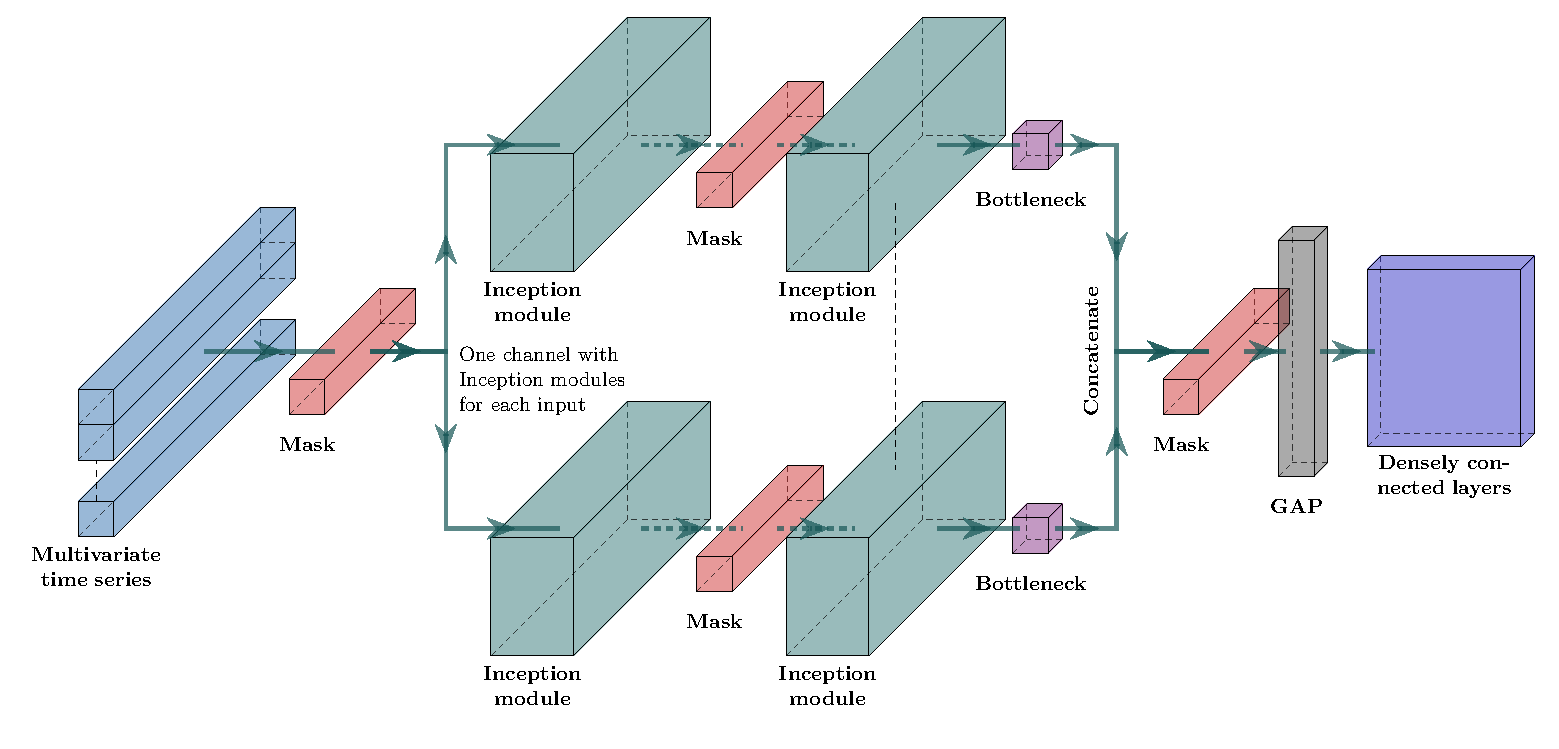
\includegraphics[width=\textwidth]{files/figs/x-inception-w-masks.pdf}
  \caption{The X-InceptionTime architecture developed in this work.}
  \label{fig:x-inception}
\end{figure}

\subsection{Training}

\subsection{Choice of input features}

\subsection{Combined score}

% !TEX root=../../mt-motion-analysis.tex
\chapter{Results} \label{ch:results}

% !TEX root=../../mt-motion-analysis.tex
\chapter{Conclusions and Discussion} \label{ch:conclusions}

\addcontentsline{toc}{chapter}{References}

\fontsize{10}{12}
\setstretch{0.9}
\printbibliography
% !TEX root=../../mt-motion-analysis.tex
\newpage
\appendix
\newpage
\etocdepthtag.toc{mtappendix}
\etocsettagdepth{mtchapter}{none}
\etocsettagdepth{mtappendix}{subsection}
\etoctocstyle{1}{Appendix - Contents}
\tableofcontents
\newpage


\chapter{POEs}
\begin{figure}[b]
  \centering
  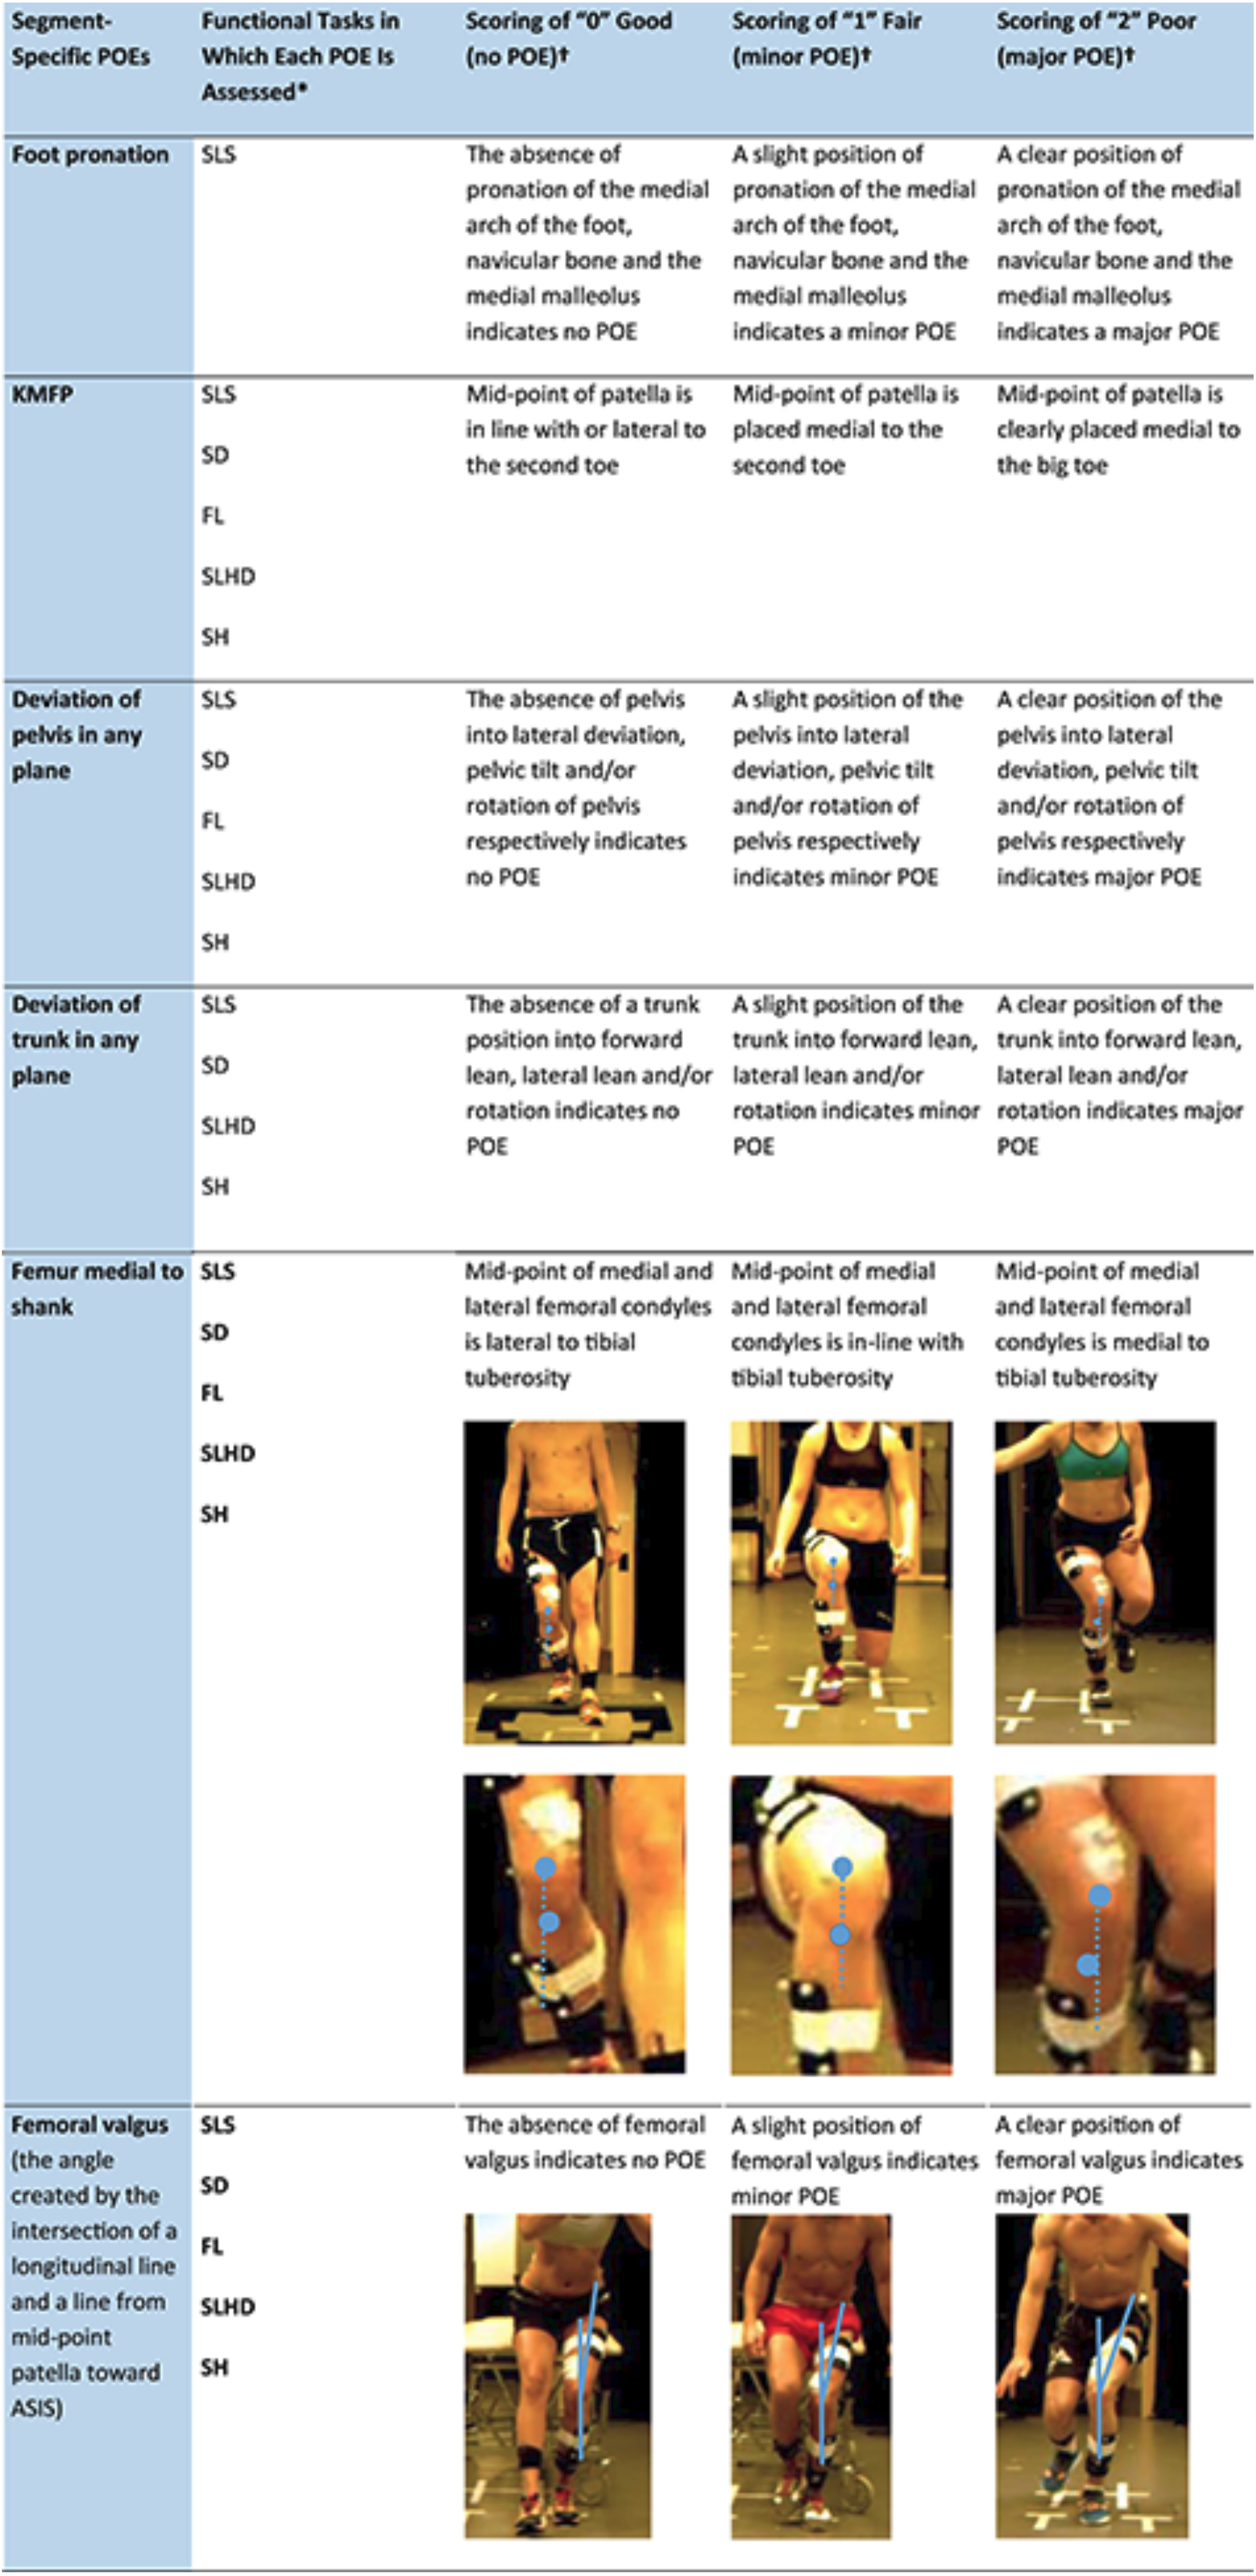
\includegraphics[height=\textheight]{files/figs/poes-detailed-rot.png}
  % \caption{}
  \label{}
\end{figure}


\chapter{wtf}
this is the information

\end{document}
